% -*- coding: utf-8 -*-
% !TEX program = xelatex
\documentclass{jnuthesis}
\usepackage{amsmath}
\usepackage{algorithmic}
\usepackage{array}
\usepackage{fixltx2e}
\usepackage{stfloats}
\usepackage{url}
\usepackage{multicol}
\usepackage{graphicx}
\usepackage{ctex}
\usepackage{subfigure}
\usepackage{float}
\usepackage{indentfirst}
\usepackage{booktabs}
\usepackage{lscape}
\usepackage{caption}
\usepackage{subfigure}
\usepackage{titlesec}
\titleclass{\chapter}{straight}
\titleformat{\chapter}[hang]  {\fontsize{12bp}{10pt}\bfseries\raggedright}{\arabic{chapter}}{1em}{}





\begin{document}
	\fontsize{10.5bp}{24pt}
	\renewcommand{\biaoti}{海上风力发电-水下压缩空气储能互补系统建模仿真与经济效益分析} 
	\renewcommand{\xingming}{余思贤、周允康、何婷}
	\XeTeXlinebreaklocale "zh"
	\XeTeXlinebreakskip = 0pt plus 1pt minus 0.1pt
	
	
	
	
	\titlepage
	\begin{zhabstract}
		\zhaiyao 将风能为代表的新能源转化为电能并应用于国民经济生产和人民生活领域成为研究热点,但是其波动性和随机性会给电网带来一定的不安全因素,所以在实际应用中,往往将随机性大波动性强的风能先转化为稳定的机械能,再进一步转化为较为清洁的电能。本研究建立了海上风力发电-水下压缩空气储能互补系统模型并以此作为研究对象,进行系统模型的仿真与分析,同时使用随机概率研究和真实数据拟合相结合的方法,对系统进行稳定性、经济性和方案可行性分析,期望将来能将新能源较有效地应用国民经济生产和人民生活领域。结果显示,该系统能将随机波动的海上风能先转化为高压空气的稳定的机械能,再进一步转化为稳定且清洁的电能,并且在随机波动的风能输入下系统循环效率和运行理论分别可达$ 69\% $和$ 11956 $元/周期,运行$ 20 $年总利润可达$ 2.85 $千万元。
		
		\guanjianci 海上风力发电-水下压缩空气储能;互补系统;能效性;经济效益分析;可行性分析。
		
	\end{zhabstract}
	%\IEEEpeerreviewmaketitle
	%\begin{multicols}{2}
	\chapter{引言}
	
	\par 在以化石能源为主体的传统能源日益枯竭的背景下,可再生能源在能源结构中的比重和作用越来越大,海洋可再生能源具有潜能巨大,靠近能源消费中心、不占宝贵土地资源,增强沿海国家能源安全等诸多优势,但相比于已经开发得较为成熟的陆上可再生资源,海上可再生资源开发仍处于初级阶段。近年来,海上风能成为国内外学者的研究热点,其中将海上风能转化为电能是研究的主要方向。然而,海上风能存在着随机性大,波动性强和能量密度低的特点,而且大规模的海上风力发电直接输入电网中容易对电网造成巨大冲击,导致电网瘫痪,影响国民经济生产和人民的日常生活,所以合适的储能技术是解决以上问题的有效方法之一。因此,压缩空气储能成为了海上能源开发尤其是海上风能开发的重要研究分支。参考传统的压缩空气储能技术,其共同点是利用电网中过剩的电能驱动空气压缩机械将常温常压状态下的空气进行压缩,并将高压空气储存在稳固可靠的密闭空间,如特制的地下气库和专门开发的密闭石洞,这种储能技术存在压缩存储过程伴随着大量的热损失和建立存储空间的高额成本等缺点。
	\par 结合海洋深处恒高压和海床面积巨大的独特条件,水下压缩空气储能技术应运而生,该技术尤其适合于沿海及海上能源的大规模存储,为未来海洋可再生能源的大规模存储提供了一种全新的思路和可行性技术方案。国内研究该新型储能技术的学者中以大连海事大学王志文博士为代表,王志文博士设计了一个多级压缩的水下压缩空气储能系统并对其进行了能效分析,其主要思路是利用电网中过剩电能驱动空气压缩机压缩空气,并将高压空气储存在海上深处的柔性储气包中,实现将电网过剩电能转化为可长期存储的空气机械能,弥补了电力系统不能长时间储存过剩电能的缺点。本文在王志文博士的研究基础上,将水下压缩空气储能技术应用到海上风能的储存中,设计了一个海上风力发电-水下压缩空气储能互补系统模型,系统的主要设计思路是利用海上风力发电机组进行发电,将海上风能转化为电能以驱动空气压缩机压缩空气,再将高压空气储存在海洋深处的柔性储气包中,用电高峰期时将高压空气膨胀释放能量,推动发电机发电,输出稳定的电能,该系统实现了将随机性大,冲击性强的海上转化为稳定的电能,克服了传统风力发电直接输入电网产生冲击的缺点,在一定程度上保障了电网安全。
	\par 能效性,即能源开发系统对能源的有效利用率是评判能源开发系统性能优劣的重要依据,因此本文在就设计的海上风力发电-水下压缩空气储能互补系统进行了能效分析。同理,经济性和可实现性也是能源系统开发的另一个重要关注点,因此本文还对所设计的系统进行了简单的经济效益分析,从经济性的角度去分析系统开发的可行性,希望供相关能源能源开发部门决策参考。
	\par 本文结构可划分为$ 6 $节,第$ 1 $节为引言,阐述本文研究的背景、思路和意义;第$ 2 $节为海上风力发电-水下压缩空气互补储能互补系统设计;第$ 3 $节阐述了本文所设计的系统热力学模型求解思路;第$ 4 $节为海上风力发电-水下压缩空气储能互补系统热力学建模与仿真;第$ 5 $节是对本文所设计的系统进行经济效益分析;第$ 6 $节为结论,对全文的研究结果进行总结。	
	
	
	\chapter{海上风力发电-水下压缩空气储能互补系统数学建模}
	\vspace{-2em} 
	\section{海上风力发电-水下压缩空气储能互补系统结构与原理}
	
	海上风力发电-水下压缩空气互补$ (OWPG-UWCAC) $系统主要由风力发电机组、空气压缩系统、空气存储装置、空气膨胀系统、换热系统以及汽轮发电机组$ 6 $个子系统构成。图$ \fontsize{10.5bp}{10pt}\ref{general system} $所示为本研究所设计的系统结构原理图。\\
	
	%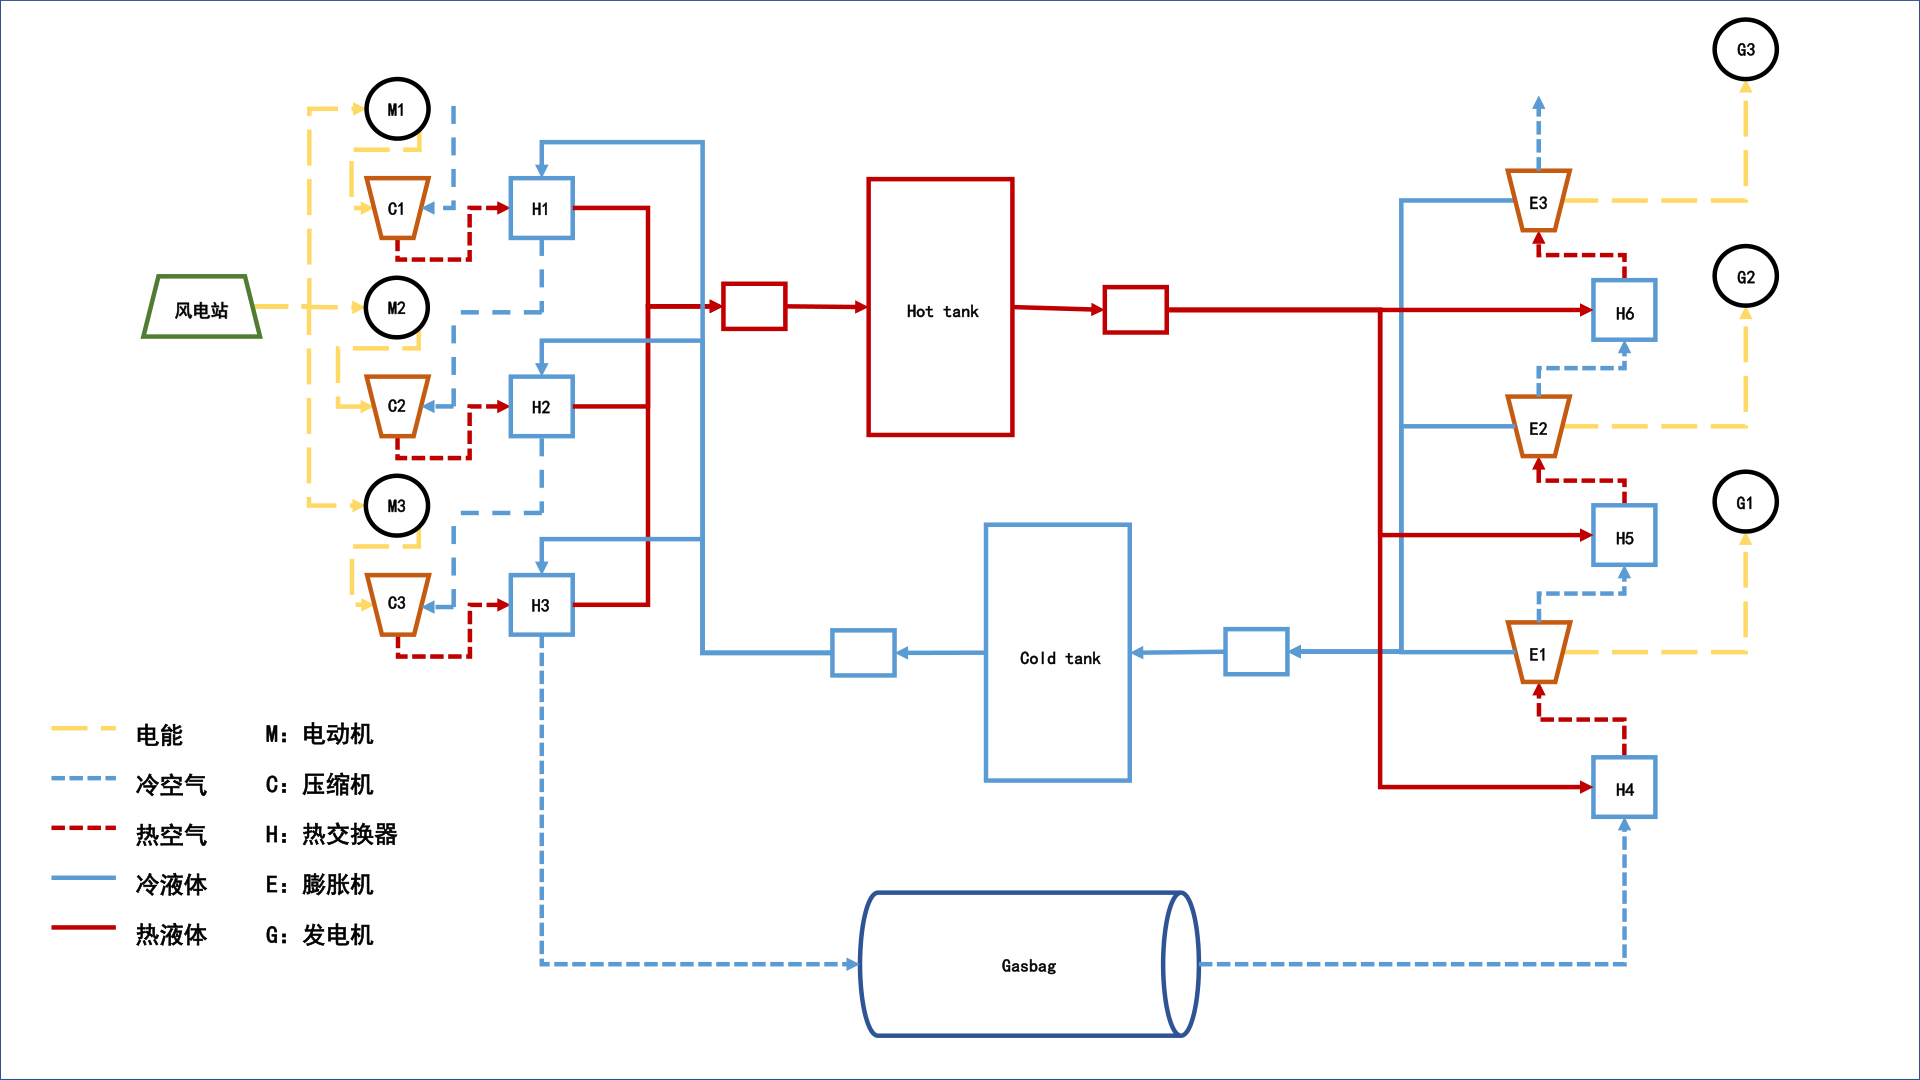
\includegraphics[scale=0.165]{pictures/The_whole_system.png}
	\begin{figure}[H] %figure环境,h默认参数是可以浮动,不是固定在当前位置。如果要不浮动,你就可以使用大写float宏包的H参数,固定图片在当前位置,禁止浮动。
		\centering %使图片居中显示
		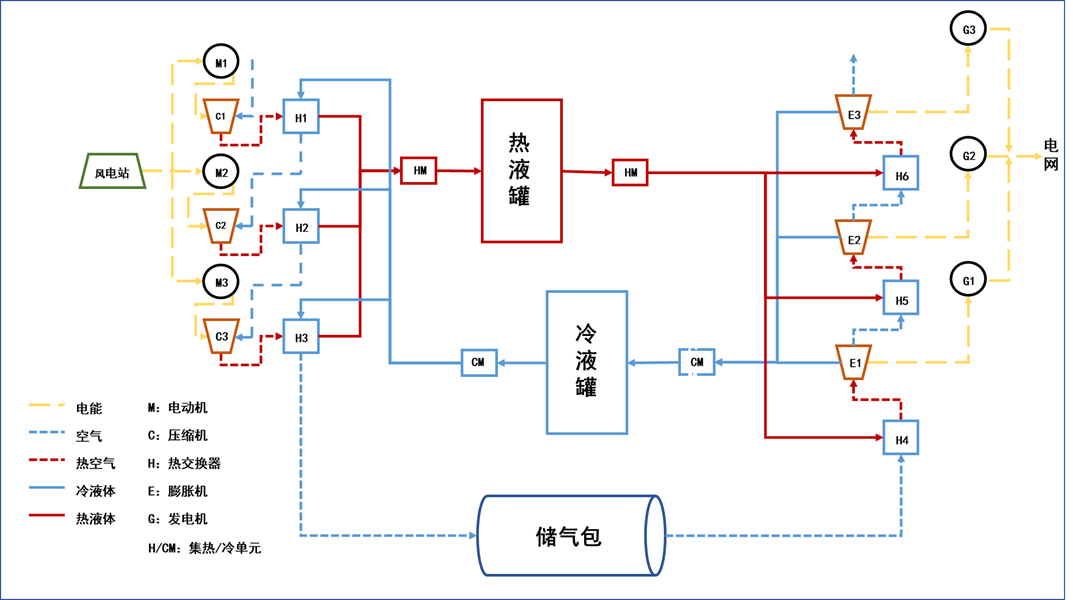
\includegraphics[width=0.8\textwidth]{pictures/screenshot001} %中括号中的参数是设置图片充满文档的大小,你也可以使用小数来缩小图片的尺寸。
		\caption{\fontsize{10.5bp}{10pt}海上风力发电-水下压缩空气储能互补系统结构图} %caption是用来给图片加上图题的
		\label{general system} %这是添加标签,方便在文章中引用图片。
	\end{figure}%figure环境
	
	
	该系统的具体工作过程如下。在储能时,风力发电机输出电能驱动电动机$ (M1,M2$和$M3) $和空气压缩机$ (C1,C2 $和$ C3) $压缩空气至较高压力状态,压缩过程中会产生大量热量,为了提高压缩机效率,降低能耗,采用三级压缩和中间冷却方法。
	\par 冷却流体(导热油)来自冷液柜$ (CT) $,冷的导热液在换热器$ (H1,H2和H3) $中冷却高温的压缩空气,之后热的导热液汇集到热液柜$ (HT) $中储存起来。压缩空气储存到储气装置$ (Gasbag) $中,对于传统定容压缩空气储能,压缩空气储存在固定容积的储气装置中,容器内气体压力随着充放气过程变化。
	\par 而对于海上风力发电-水下压缩空气储能互补系统,压缩空气的压力保持不变,储气装置内储气容积变化。在需要释能发电时,储气装置内的压缩空气释放出来,高温导热液储存柜中储存的导热液进入到换热器$ (H4,H5,H6) $内与压缩空气进行热交换,高温高压空气驱动空气膨胀机$ (E1,E2,E3) $和发电机$ (G1,G2 $和$ G3) $发电。空气膨胀装置采用三级膨胀和中间加热方式提高发电效率。
	
	
	
	
	
	\section{海上风力发电-水下压缩空气储能互补系统的热力学模型}
	\subsection{海上风力发电机}
	
	海上风力发电机组是本系统将自然界的风能转化为电能的装置,因为海风具有随机性和波动性,随机性表现为海面上有无风的不确定性,波动性表现为风速大小的不稳定性,从而导致风力发电机组输出的电能具有随机性和波动性,即有无电能输出的不确定性和输出功率大小的不稳定性。结合目前风力发电发展现状,本文的海上风力发电机组模型,采用了对桂山海上风电场一个月的风电功率数据进行拟合,将总体风电功率划分为$ 10 $个等级,如表$ \fontsize{10.5bp}{10pt}\ref{wind_power} $所示,并求出相应概率,通过指定概率的随机函数来进行对单次风电功率的拟合。
	
	%https://www.tablesgenerator.com/ 做表格用这个
	% Please add the following required packages to your document preamble:
	% \usepackage{booktabs}
	% \usepackage{graphicx}
	
	\begin{table}[H]
		\centering
		\resizebox{\textwidth}{!}{%
			\begin{tabular}{@{}l|llllllllll@{}}
				\toprule
				风功率等级 & $\rho_{wind}^1$ & $\rho_{wind}^2$ & $\rho_{wind}^3$ & $\rho_{wind}^4$ & $\rho_{wind}^5$ & $\rho_{wind}^6$ & $\rho_{wind}^7$ & $\rho_{wind}^8$ & $\rho_{wind}^9$ & $\rho_{wind}^{10}$ \\ \midrule
				概率 & 0.06 & 0.11 & 0.13 & 0.11 & 0.07 & 0.15 & 0.15 & 0.06 & 0.11 & 0.05 \\ \bottomrule
			\end{tabular}%
		}
		\caption{\fontsize{10.5bp}{10pt}风功率等级及其概率\cite{b8}}
		\label{wind_power}
	\end{table}
	
	考虑到实际情况,风电功率虽然是突变的,但一般情况下每$ 5 $分钟内的风电功率并不会大幅度上升或下降,因此人为指定了相邻两次风电功率等级之间差值不超过$ 2 $,以此来反映真实情况。如图$ \fontsize{10.5bp}{10pt}\ref{fig:screenshot002} $所示为较为接近现实情况的海上风力发电机组模型。
	
	
	\begin{figure}[H]
		\centering
		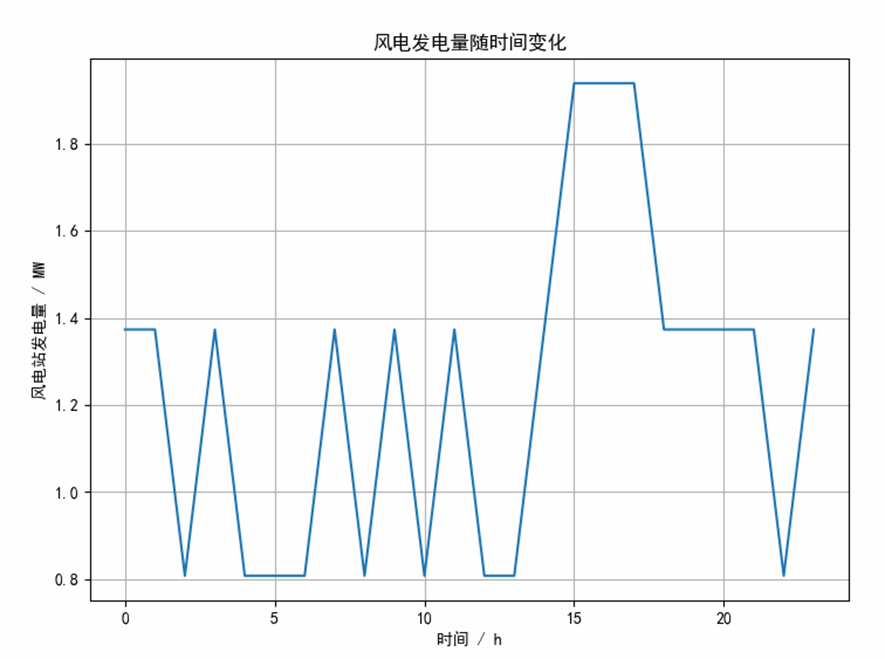
\includegraphics[width=0.7\linewidth]{pictures/screenshot002}
		\caption{\fontsize{10.5bp}{10pt}海上风力发电机组模型输出功率图}
		\label{fig:screenshot002}
	\end{figure}
	
	
	\subsection{空气压缩机和空气膨胀机}\ 
	
	压缩机和膨胀机是该系统的关键装置,其种类较多,本系统拟采用离心式压缩机和膨胀机。假设各级压缩机有相同的压缩比和各级膨胀机有相同的膨胀机之下,用等熵效率评价透平机械的能效。
	\par 压缩机实际压缩终温为:
	
	\begin{equation}
		T_{f, \text { comp }}=T_{\text {in }}\left[1+\frac{1}{\eta_{\text {comp }}}\left(\frac{p_{f}}{p_{i}}\right)^{\frac{r-1}{r}}\right]
	\end{equation}
	
	
	膨胀机实际膨胀终温为:
	\begin{equation}
		T_{f, \exp }=T_{\text {in }}\left\{1-\eta_{\exp }\left[1-\left(\frac{p_{f}}{p_{i}}\right)^{\frac{r-1}{r}}\right]\right\}
		\label{f2}
	\end{equation}
	
	
	压缩机的各级压缩比:\\
	
	\begin{equation}
		\beta_{\text {comp }}=\frac{P_{\text {out }}}{P_{\text {in }}}=\sqrt[3]{\frac{\rho g h }{P_{\text {atm }} }}
	\end{equation}\ 
	
	膨胀机的各级膨胀比:\\
	
	\begin{equation}
		\beta_{\text {exp }}=\frac{P_{\text {out }}}{P_{\text {in }}}=\sqrt[3]{\frac{\rho g h }{P_{\text {atm }} }}
	\end{equation}\ 
	
	系统各个环节空气质量守恒(即不考虑气动管路微量损失),可知压缩机和膨胀机不考虑可变导叶的影响,因此,透平机械实际效率可以认为是实际流量和实际压缩比的函数:
	\begin{equation}
		\eta=f(m, \beta)
		\label{f5}
	\end{equation}
	
	将式$ (\fontsize{10.5bp}{10pt}\ref{f5}) $多项式展开可表达为:
	\begin{equation}\label{f6}
		\eta_{\text {actual }}=a_{1}+a_{2} m_{\text {actual }}+a_{3} \beta_{\text {actual }}+a_{4} m_{\text {actual }} \beta_{\text {actual }}+a_{5} m_{\text {actual }}^{2}+a_{6} \beta_{\text {actual }}^{2}+a_{7} m_{\text {actual }}^{2} \beta_{\text {actual }}^{2}
	\end{equation}
	
	
	假设压缩机/膨胀机额定流量为 $ m_{rated}$,额定压缩比/膨胀比为 $ \beta_{rated}$,设计工况点的额定效率为$\eta_{designed}$。定义无量纲化的流量比、压力比/膨胀比和效率分别为:
	
	\begin{equation}\label{f7}
		m_{n}=\frac{m_{\text {actual }}}{m_{\text {rated }}}
	\end{equation}
	
	\begin{equation}\label{f8}
		\beta_{n}=\frac{\beta_{\text {actual }}}{\beta_{\text {rated }}}
	\end{equation}
	
	\begin{equation}\label{f9}
		m_{n}=\frac{\eta_{\text {actual }}}{\eta_{\text {rated }}}
	\end{equation}
	
	则结合定义式$  (\fontsize{10.5bp}{10pt}\ref{f7}) (\fontsize{10.5bp}{10pt}\ref{f8}) (\fontsize{10.5bp}{10pt}\ref{f9})  $,式$ (\fontsize{10.5bp}{10pt}\ref{f6}) $:
	
	\begin{equation}\label{f10}
		\eta_{n}=b_{1}+b_{2} m_{n}+b_{3} \beta_{n}+b_{4} m_{n} \beta_{n}+b_{5} m_{n}^{2}+b_{6} \beta_{n}^{2}+b_{7} m_{n}^{2} \beta_{n}^{2}
	\end{equation}
	
	在式$ (\fontsize{10.5bp}{10pt} $\ref{f10})中,$  \quad b_{1}=-0.03548, \quad b_{2}=0.1528811, \quad b_{3}=1.936395,b_{4}=0.1096184, \quad b_{5}=-0.1302482, \quad b_{6}=-1.0224731, \quad b_{7}=-0.0107012 $ \cite{b3}
	
	则式$ (\fontsize{10.5bp}{10pt}\ref{f10}) $为图$ \fontsize{10.5bp}{10pt}\ref{fig3a} $所示:
	
	
	对于透平机械而言,空气压力损失会造成透平机械的压缩比/膨胀比略微减小,在本系统中,连接各环节的气动管路造成微小的压力损失,约为 $ 0\sim 1 k P a $,远小于空气压强,故可忽略不计,因此压缩比和膨胀比的无量纲物理量$ \beta_{n} \approx 1 $,式$ (\fontsize{10.5bp}{10pt}\ref{f10}) $可化简为式$ (\fontsize{10.5bp}{10pt}\ref{f11}) $。此时,图$ \fontsize{10.5bp}{10pt}\ref{fig3a} $可转换为图$ \fontsize{10.5bp}{10pt}\ref{fig3b} $。
	
	\begin{equation}\label{f11}
		\eta_{n}=b_{1}+b_{2} m_{n}+b_{3}+b_{4} m_{n}+b_{5} m_{n}^{2}+b_{6}+b_{7} m_{n}^{2}
	\end{equation}
	
	压缩机/膨胀机对空气做的压缩功率/膨胀功率可根据式$ (\fontsize{10.5bp}{10pt}\ref{f12}) $计算:
	\begin{equation}\label{f12}
		P_{\text {comp }}=m_{\text {compressor }}\left(H_{\text {out }}-H_{\text {in }}\right) P_{\text {expander }}=m_{\text {expander,air }}\left(H_{\text {in }}-H_{\text {out }}\right)
	\end{equation}
	
	其中$ H $为空气的焓值,可由式$ (\fontsize{10.5bp}{10pt}\ref{f13}) $计算:
	
	\begin{equation}\label{f13}
		H_{a i r}=4.6020+0.9705 T+3.3955 \times 10^{-5} T^{2}+3.3955 \times 10^{-8} T^{3}+1.697 \times 10^{-11} T^{4}
	\end{equation}
	\begin{figure}[H]
		
		\subfigure[典型的透平机械无量纲化的效率图] %第一张子图
		{
			\begin{minipage}{0.5\linewidth}
				\centering          %子图居中
				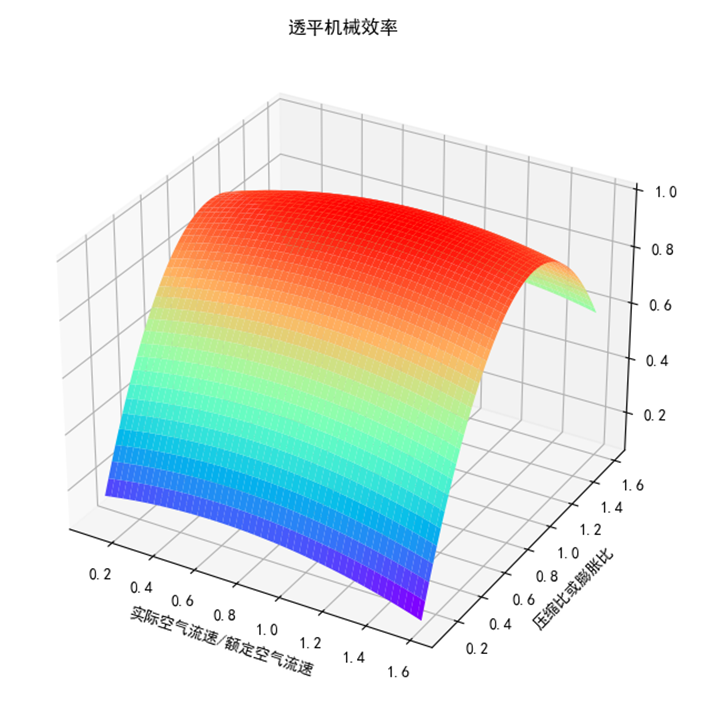
\includegraphics[width=0.9\linewidth]{pictures/screenshot003}
				\label{fig3a}   %以pic.jpg的0.5倍大小输出
			\end{minipage}
		}
		\subfigure[典型透平机械效率与空气质量流量无量纲量关系图] %第二张子图
		{
			\begin{minipage}{0.5\linewidth}\label{b}
				\centering      %子图居中
				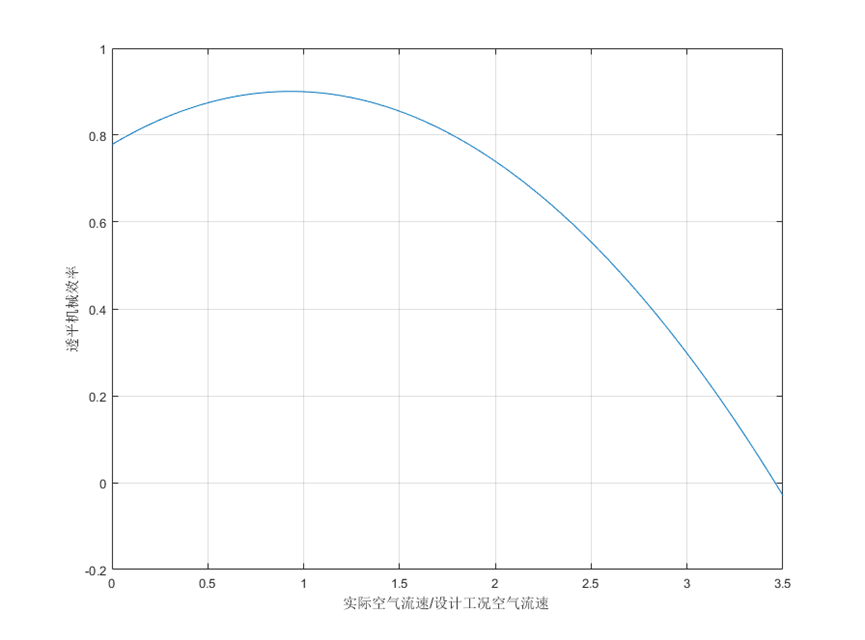
\includegraphics[width=0.9\linewidth]{pictures/screenshot004}
				\label{fig3b}   %以pic.jpg的0.5倍大小输出
			\end{minipage}
		}
		
		
		\caption{\fontsize{10.5bp}{10pt}式$ (\fontsize{10.5bp}{10pt}\ref{f10}) $和式$ (\fontsize{10.5bp}{10pt}\ref{f11}) $} %  %大图名称
		\label{fig:3}  %图片引用标记
	\end{figure}
	
	
	\subsection{换热系统}
	
	换热系统是由换热器和储热单元组成的,其中,换热器是联接压缩/膨胀空气子系统的核心设备,换热器的性能通常用有效度来衡量,有效度定义为实际换热量与最大可能换热量的比值:\\
	
	\begin{equation}\label{f14}
		\epsilon=\frac{\dot{Q}_{actual}}{\dot{Q}_{max}}=\frac{(\dot{m}c_p\Delta T)_{cold \  or \  hot}}{(\dot{m}c_p)_{min}(T_{hot,in}-T_{cold,in})}
	\end{equation}
	
	其中$ \left(\dot{m}{c_{p}}\right)_{\min } $表示热流体和冷流体热熔率中的小者。
	\par 在本系统中,规定$ \epsilon=0.9 $。
	\par 假设某级压缩机对空气做压缩功$ W_{\text {comp},i}(i=1,2,3) $,使得空气内能增加量为$ \Delta Q_{\text {comp}, i}(i=1,2,3) $,则经过与换热器中的低温导热油换热后,空气温度可由式$ (\fontsize{10.5bp}{10pt}\ref{f15}) $计算:
	\begin{equation}\label{f15}
		c_{a i r} m_{a i r}\left(T_{i n, a i r}-T_{o u t, a i r}\right)=\epsilon \Delta Q_{c o m p, i}(i=1,2,3)
	\end{equation}
	
	其中,$ c_{a i r} $为空气比热容,可由式$ (\fontsize{10.5bp}{10pt}\ref{f16}) $计算:
	
	\begin{equation}\label{f16}
		c_{a i r}=0.9705+6.791 \times 10^{-5} T+1.658 \times 10^{-7} T^{2}-6.788 \times 10^{-11} T^{3}
	\end{equation}
	
	导热油吸收热量后经储热小单元汇聚到储热罐中储存起来,其中储热罐是利用热绝缘材料建造的,热量损失可以忽略不计。储热罐中导热油可由式$ (\fontsize{10.5bp}{10pt}\ref{f17}) $计算:
	
	\begin{equation}\label{f17}
		\sum \epsilon \Delta Q_{\text {comp },i}=c_{\text {oil }} m_{\text {oil }}\left(T_{\text {out }, \text { oil }}-T_{\text {in,oil }}\right)(i=1,2,3)
	\end{equation}
	
	其中,$ c_{\text {oil }} $为导热油比热容,可由式$ (\fontsize{10.5bp}{10pt}\ref{f18}) $计算:
	\begin{equation}\label{f18}
		c_{o i l}=1.2266+0.0014(T-273.15)
	\end{equation}
	
	对于与膨胀机相连的换热器,空气经过与换热器中的高温导热油换热后,空气温度可由式$ (\fontsize{10.5bp}{10pt}\ref{f19}) $计算:
	
	\begin{equation}\label{f19}
		T_{\text {air,hot }}=T_{\text {air,cold }}+\epsilon \frac{\left(\dot{m} c_{p}\right)_{\min }}{\left(\dot{m} c_{p}\right)_{\text {air }}}\left(T_{\text {oil,hot }}-T_{\text {air,cold }}\right)
	\end{equation}
	
	换热完成后,导热油流入冷液罐储存起来,其中冷液罐是采用导热性良好的材料建造的,温度可保持与所处海域温度相同,暂定为$ 290K $
	
	
	\subsection{空气储存装置}
	
	
	空气储存装置的作用为存储压缩空气,本系统拟采用圆球状柔性储气装置,利用水的静压特性对压缩空气实现定压存储,储气装置内压缩空气温度和压强与所处水体位置的温度与压强基本一致。
	\par 
	压缩空气温度可由式$ (\fontsize{10.5bp}{10pt}\ref{f20}) $计算:
	
	\begin{equation}
		T_{gasbag}=T_{water}
		\label{f20}
	\end{equation}
	
	压缩空气压强可由式$ (\fontsize{10.5bp}{10pt}\ref{f21}) $计算:\\
	\begin{equation}
		P_{air,gasbag}=P_{water}=\rho_{water}gh
		\label{f21}
	\end{equation}
	
	\subsection{电动机和发电机}
	
	
	如图$ \fontsize{10.5bp}{10pt}\ref{general system} $所示,系统中共有三台电动机和三台发电机,其耗电/发电功率分别由式$ (\fontsize{10.5bp}{10pt}\ref{f22}) $和式$ (\fontsize{10.5bp}{10pt}\ref{f23}) $计算:
	
	\begin{equation}
		W_{\text {motor }}=c_{i} W_{\text {wind }}(i=1,2,3)
		\label{f22}
	\end{equation}
	\begin{equation}
		W_{\text {generator},i}=\eta_{\text {generator }} W_{\text {expander},i}(i=1,2,3)
		\label{f23}
	\end{equation}
	
	其中,$ c_i  $为风电能分配比例,本系统暂定$ c_{1}=32.24 \%, \quad c_{2}=33.06 \%, \quad c_{3}=34.7 \% $。
	$ \eta_{\text {generator }} $为发电机$ G1,G2,G3 $的发电效率,暂定$ \eta_{\text {generator }} =95\%$
	
	
	系统电动机耗电总功率和发电机发电总功可由式$ (\fontsize{10.5bp}{10pt}\ref{f24}) $和式$ (\fontsize{10.5bp}{10pt}\ref{f25}) $计算:
	
	\begin{equation}
		W_{motor,total}=W_{motor,1}+W_{motorr,2}+W_{motor,3}
		\label{f24}
	\end{equation}
	\begin{equation}
		W_{generator,total}=W_{generator,1}+W_{generator,2}+W_{generator,3}
		\label{f25}
	\end{equation}
	
	
	
	\chapter{系统热力学模型求解}
	\par 海上风力发电-水下压缩空气储能互补系统运行可以分为四种基本工作过程:海上风力发电过程、压缩储能过程、存储过程和膨胀释能过程。海上风力发电机将风能转化为电能驱动电动机来带动压缩机压缩空气进行储能,存储压缩空气和高温导热液;膨胀释能过程释放存储的压缩空气驱动膨胀机和发电机发电,同时释放导热液存储的热能。
	在$ Python $中建立系统模型进行求解。系统基本参数如$ 表\fontsize{10.5bp}{10pt}\ref{tab:my-table} $所示。
	
	\begin{table}[]
		\centering
		\resizebox{\textwidth}{!}{
			\begin{tabular}{l|c|r|l|c|r}
				\multicolumn{1}{c|}{参数} & 单位                      & \multicolumn{1}{c}{数值(基准值)} &\multicolumn{1}{|c|}{参数} & 单位                      & \multicolumn{1}{c}{数值(基准值)} \\ \hline
				&                     &                      &                 &                       & \\
				大气压力$ P_{atm} $                    & Pa                      & 101325                      &膨胀势能总时间                 & 小时                      & 3\\
				大气温度$ T_{atm} $                    & K                       & 298.15                      &膨胀机1额定等熵效率              & \%                      & 90 \\
				额定空气流速                  & kg/s                    & 8.5                         &膨胀机2额定等熵效率              & \%                      & 90\\
				风电站额定输出功率               & MW                      & 2.45                        &膨胀机3额定等熵效率              & \%                      & 90\\
				电动机M1额定输入效率             & \%                      & 90                          &膨胀机1额定膨胀比               &                         & 2.1544\\
				电动机M2额定输入效率             & \%                      & 90                          &膨胀机2额定膨胀比               &                         & 2.1544\\
				电动机M3额定输入效率             & \%                      & 90                         &膨胀机3额定膨胀比               &                         & 2.1544 \\
				电动机M1额定输入功率             & MW                      & 0.79                        &膨胀机1膨胀功率                & MW                      & 1.76 \\
				电动机M2额定输入功率             & MW                      & 0.81                        &膨胀机2膨胀功率                & MW                      & 1.77\\
				电动机M3额定输入功率             & MW                      & 0.84                        &膨胀机3膨胀功率                & MW                      & 1.77\\
				压缩机1额定等熵效率              & \%                      & 90                          &发电机1额定发电效率              & \%                      & 95\\
				压缩机2额定等熵效率              & \%                      & 90                         &发电机2额定发电效率              & \%                      & 95\\
				压缩机3额定等熵效率              & \%                      & 90                          &发电机3额定发电效率              & \%                      & 95\\
				压缩机1额定等压缩比              &                         & 2.1544                     &发电机1额定输出功率              & MW                      & 1.67 \\
				压缩机2额定等压缩比              &                         & 2.1544                      &发电机2额定输出功率              & MW                      & 1.68\\
				压缩机3额定等压缩比              &                         & 2.1544                      &发电机3额定输出功率              & MW                      & 1.68\\
				压缩储能总时间                 & H                       & 9                         &换热器额定有效度                &                         & 0.9  \\
				额定水下储存深度                & m                       & 100                        &换热器1额定换热功率              & MW                      & 0.64  \\
				储存压强                    & Pa                      & 1013201                    &换热器2额定换热功率              & MW                      & 0.68 \\
				储存空气总质量                 & kg                      & 275400                      &换热器3额定换热功率              & MW                      & 0.68\\
				额定空气密度                  & $ kg/m^3 $ & 11                         &换热器4额定换热功率              & MW                      & 2.27 \\
				储存空气总体积                 & $ m^3  $   & 25036.4                    &换热器5额定换热功率              & MW                      & 1.81 \\
				储气包规格                   & $ m^3 $    & 30000                      &换热器6额定换热功率              & MW                      & 1.77  \\
				存储时间                    & 小时                      & 3                          &压缩过程导热油流速/空气流速          & kg/s                    & 1.7  \\
				额定膨胀空气流速                & kg/s                    & 25.5                        &膨胀过程导热油流速/空气流速          & kg/s                    & 1.7  \\
				储热罐额定温度                 & K                       & 388                         &系统循环效率                  & \%                      & 68.46\\
				冷液罐额定温度                 & K                       & 290                         
				
			\end{tabular}
		}
		\caption{\fontsize{10.5bp}{10pt}系统额定工况条件运行相关参数}
		\label{tab:my-table}
	\end{table}
	
	\par 压缩储能过程电能总消耗量可由式$ (\fontsize{10.5bp}{10pt}\ref{f31}) $计算:
	\begin{equation}\label{f31}
		W_{\text {motor,total }}=W_{\text {motor }, 1}+W_{\text {motorr }, 2}+W_{\text {motor }, 3}=\int_{0}^{t_{1}}\left(P_{m 1}+P_{m 2}+P_{m 3}\right) d t
	\end{equation}
	
	
	\par 其中,$ t_1 $为压缩空气所耗费的时间。
	\par 膨胀释能过程生产的总电能可由式$ (\fontsize{10.5bp}{10pt}\ref{f32}) $计算:
	\begin{equation}\label{f32}
		W_{\text {generator,total }}=W_{\text {generator, } 1}+W_{\text {generator, } 2}+W_{\text {generator }, 3}=\int_{0}^{t_{2}}\left(P_{G 1}+P_{G 2}+P_{G 3}\right) d t
	\end{equation}
	
	其中,$ t_2 $为膨胀释能所耗费的时间。
	\par 系统效率可由式$ (\fontsize{10.5bp}{10pt}\ref{f33}) $计算:
	
	
	\begin{equation}\label{f33}
		\begin{aligned}
			\eta_{\text {system }}&=\frac{W_{\text {generator,total }}}{W_{\text {motor,total }}}=\frac{\int_{0}^{t_{2}}\left(P_{G 1}+P_{G 2}+P_{G 3}\right) d t}{\int_{0}^{t_{1}}\left(P_{m 1}+P_{m 2}+P_{m 3}\right) d t}
			\\
			&=\frac{\int_{0}^{t_{2}} \eta_{\text {generator }}\left(P_{\text {expander } 1}+P_{\text {expander } 2}+P_{\text {expanders }}\right) d t}{\int_{0}^{t_{1}}\left(P_{\text {wind }}\right) d t}\\
			&=\frac{\int_{0}^{t_{2}} \eta_{\text {generator }}\left(m_{\text {expander,air} }(H_{in,4}-H_{out,4})+m_{\text {expander,air} }(H_{in,5}-H_{out,5})+m_{\text {expander,air} }(H_{in,6}-H_{out,6})\right) d t}{\int_{0}^{t_{1}}\left(P_{\text {wind }}\right) d t}
		\end{aligned}
	\end{equation}
	
	
	因为$\int_{0}^{t_{2}} m_{\text {expander,air }}=\int_{0}^{t_{1}} m_{\text {compressor, air }}  $,故式$ (\fontsize{10.5bp}{10pt}\ref{f33}) $可变换为式$ (\fontsize{10.5bp}{10pt}\ref{f34}) $:
	
	\begin{equation}\label{f34}
		\begin{aligned}
			\eta_{\text {system }}&=\frac{\left(\left(H_{\text {in,expander } 1}-H_{\text {out } 4, \text { expander } 1}\right)+\left(H_{\text {in, expander } 2}-H_{\text {out,expander } 2}\right)+\left(H_{\text {in,expander } 3}-H_{\text {out,expander3 }}\right)\right) }{\int_{0}^{t_{1}}\left(P_{\text {wind }}\right) d t}\\ 
			&\times \eta_{\text {generator }} \int_{0}^{t_{1}} m_{\text {compressor,air}} d t
		\end{aligned}
	\end{equation}
	
	\par 本系统的膨胀释能子系统的空气流速$ m_{\text {expander, air }} $可固定在某一稳定值附近,因此可近似认为:\\
	$ \left(H_{\text {in,expander } 1}-H_{\text {out } 4, \text { expander } 1}\right)+\left(H_{\text {in, expander } 2}-H_{\text {out,expander } 2}\right)+\left(H_{\text {in,expander } 3}-H_{\text {out,expander3 }}\right) $为某一固定值,即可将焓差近似认为是某一固定值。
	\par 根据式$ (\fontsize{10.5bp}{10pt}\ref{f13}) $:焓差是关于温差的函数,所以该焓差与膨胀机$ 1,2,3 $的膨胀终温和换热器$ 4,5,6 $的出口温度之差有关。首先讨论与膨胀终温有关的因素,根据式$ (\fontsize{10.5bp}{10pt}\ref{f2}) $,膨胀终温与膨胀比和膨胀效率有关,图$ \fontsize{10.5bp}{10pt}\ref{fig4a} $所示为膨胀比和膨胀效率与膨胀机膨胀终温的关系;因为气动管路压力损失可忽略不计,故膨胀比近似额定膨胀比,膨胀机出口温度与入口温度比值如图$ \fontsize{10.5bp}{10pt}\ref{fig4b} $所示可近似关于膨胀机效率的一次函数。由图$ \fontsize{10.5bp}{10pt}\ref{fig4b} $可知,膨胀机膨胀效率越大,膨胀机出入口温度比值越小。其次讨论与换热器$ 4,5,6 $出口温度有关的因素,根据式$ (\fontsize{10.5bp}{10pt}\ref{f19}) $,换热器$ 4,5,6 $出口温度与高温导热油的温度成正比,根据式$ (\fontsize{10.5bp}{10pt}\ref{f17}) $,可得式$ (\fontsize{10.5bp}{10pt}\ref{f35}) $:
	
	\begin{figure}[H]
		\subfigure[膨胀机出入口温度比值与膨胀比和膨胀机膨胀效率关系] %第一张子图
		{
			\begin{minipage}{0.5\linewidth}
				\centering          %子图居中
				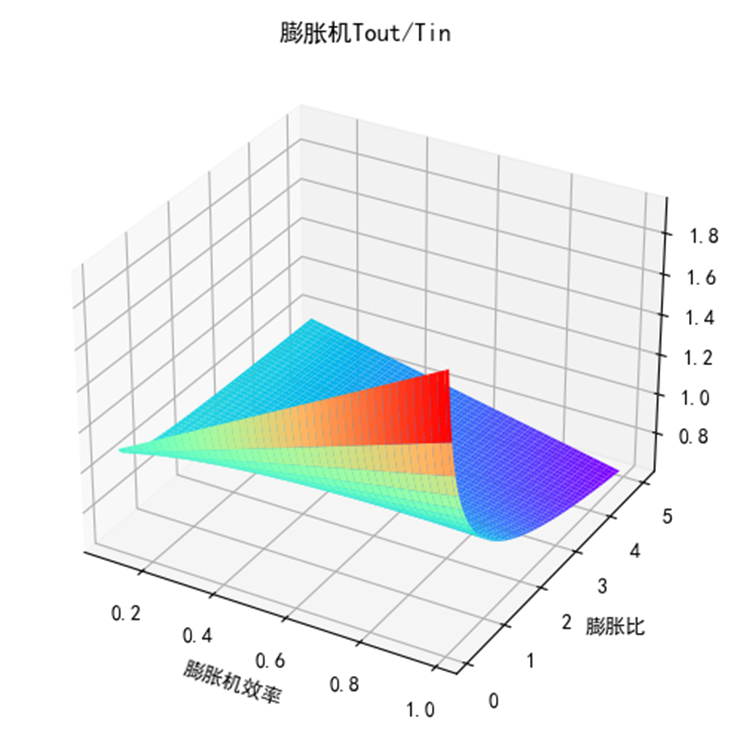
\includegraphics[width=0.9\linewidth]{pictures/screenshot005}
				\label{fig4a}   %以pic.jpg的0.5倍大小输出
			\end{minipage}
		}
		\subfigure[膨胀机出入口温度比值与膨胀机效率关系(忽略膨胀比的微小变化)] %第一张子图
		{
			\begin{minipage}{0.5\linewidth}
				\centering          %子图居中
				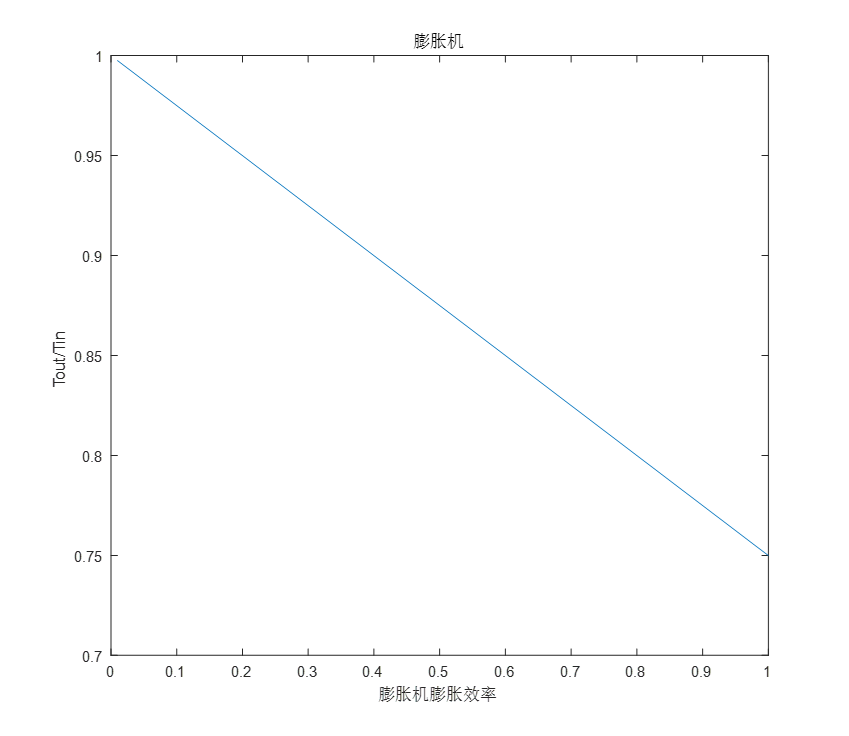
\includegraphics[width=0.9\linewidth]{pictures/screenshot006}
				\label{fig4b}   %以pic.jpg的0.5倍大小输出
			\end{minipage}
		}
		\subfigure[压缩机出入口温度比值与压缩比和压缩效率关系] %第一张子图
		{
			\begin{minipage}{0.5\linewidth}
				\centering          %子图居中
				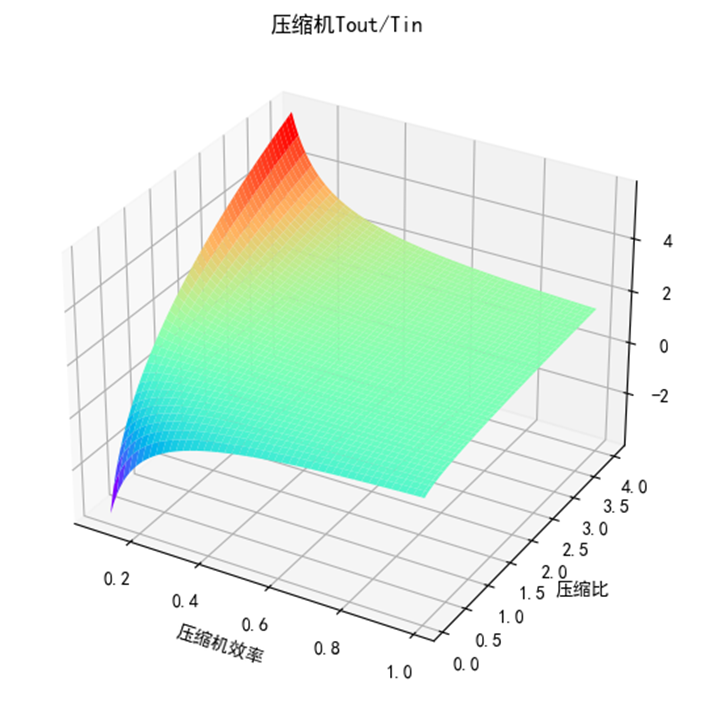
\includegraphics[width=0.9\linewidth]{pictures/screenshot007}
				\label{fig4c}   %以pic.jpg的0.5倍大小输出
			\end{minipage}
		}
		\subfigure[压缩机出入口温度比值与压缩比和压缩效率关系] %第一张子图
		{
			\begin{minipage}{0.5\linewidth}
				\centering          %子图居中
				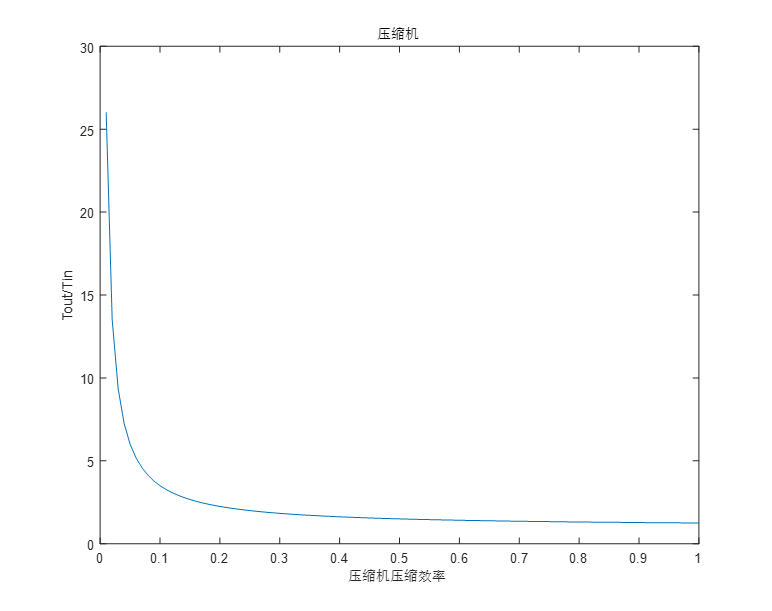
\includegraphics[width=0.9\linewidth]{pictures/screenshot008}
				\label{fig4d}   %以pic.jpg的0.5倍大小输出
			\end{minipage}
		}
		\caption{\fontsize{10.5bp}{10pt}压缩机和膨胀机的效率关系} %  %大图名称
		\label{fig:4}  %图片引用标记
		
	\end{figure}
	\begin{equation}\label{f35}
		\begin{aligned}
			&T_{\text {out,oil }}=T_{\text {in,oil }}+\epsilon \cdot m_{\text {compressor, air }}\\
			&\times \frac{\left(H_{\text {out }, \text { compressor } 1}-H_{\text {in, compressor } 1}\right)+\left(H_{\text {out }, \text { compressor } 2}-H_{\text {in, compressor } 2}\right)+\left(H_{\text {out, } \text { compressor } 3}-H_{\text {in, compressor } 3}\right)}{m_{\text {oil }}}
		\end{aligned}
	\end{equation}
	
	\par 可见,高温导热油的温度与$ \frac{m_{\text {compressor,air }}}{m_{\text {oil }}} $和$\left(H_{\text {out }, \text { compressor } 1}-H_{\text {in, compressor } 1}\right)+\left(H_{\text {out }, \text { compressor } 2}-H_{\text {in, compressor } 2}\right)+\left(H_{\text {out, } \text { compressor } 3}-H_{\text {in, compressor } 3}\right)  $有关。
	\par 其中:与$ \frac{m_{\text {compressor,air }}}{m_{\text {oil }}} $越大,$ T_{\text {out }, \text { oil }} $越大。
	\par $\left(H_{\text {out }, \text { compressor } 1}-H_{\text {in, compressor } 1}\right)+\left(H_{\text {out }, \text { compressor } 2}-H_{\text {in, compressor } 2}\right)+\left(H_{\text {out, } \text { compressor } 3}-H_{\text {in, compressor } 3}\right)  $与压缩机的压缩比和压缩效率有关,图$ \fontsize{10.5bp}{10pt}\ref{fig4c} $所示为压缩比和压缩效率与压缩机压缩终温的关系;因为气动管路压力损失可忽略不计,故压缩比近似额定压缩比,压缩机出口温度和入口温度的比值如图$ \fontsize{10.5bp}{10pt}\ref{fig4d} $所示可近似于压缩机效率的反比例型函数。由图$ \fontsize{10.5bp}{10pt}\ref{fig4d} $可知,压缩机出入口温度比值与压缩效率成反比。
	
	\par 综上所述,影响海上风力发电-水下压缩空气储能互补系统效率的主要因素有:
	\begin{itemize}
		\item 压缩比和压缩效率
		\item 膨胀比和膨胀效率
		\item 风力发电机输出功率
		\item 压缩过程空气质量流量和导热油质量流量的比值,即$ \frac{m_{\text {compressor,air }}}{m_{\text {oil }}} $
	\end{itemize}
	
	\par 若想提高系统效率,可从提高压缩比、压缩效率和$ \frac{m_{\text {compressor,air }}}{m_{\text {oil }}} $入手。通常情况下采用提高压缩比的措施。
	
	\chapter{海上风电-水下压缩空气储能互补系统不同工况运行特性}
	
	
	\par 通常系统运行工况可以分为额定设计工况和非设计工况两种。设计下系统性能是比较优越的,系统各组件通常工作在设计工况点,储存的能量利用率也通常较高,所以系统效率也是较高的。因此,通常希望系统能够保持在设计工况点或设计工况点附近运行,从而获得最佳的系统效率和工作性能。但是,在某些情况下系统会不可避免地工作在非设计工况,这在供能和负荷波动的储能系统中表现得尤为突出。对于这类非设计工况工作比例很大的系统而言,研究其非设计工况系统特性对系统的设计优化是十分重要和有必要的。本小节研究水下压缩空气储能系统在设计工况和非设计工况下的运行特性,并进行对比分析。
	
	\section{系统设计工况运行}
	
	\par 系统设计工况一个完整的运行周期包括:
	\begin{itemize}
		\item 储能:压缩储能设备以设计工况运行完成对储气装置的完全充气
		\item 存储:能量存储过程
		\item 释放能量:膨胀发电设备以设计工况运行将储气装置内的压缩空气完全释放
	\end{itemize}
	
	\par 系统基本参数以表$ \fontsize{10.5bp}{10pt}\ref{tab:my-table} $为参考,暂定一个周期内压缩储能阶段持续约$ 9 $小时,中间进行$ 3 $小时的存储过程,释放能量过程持续约$ 3 $小时。释放能量过程持续时间远小于储能持续时间是因为发电功率远大于用电功率,且系统循环效率必然地小于$ 100\% $。另外,本系统存储能量过程的少量气体损失忽略不计。
	
	\begin{figure}[h]
		\subfigure[系统设计工况条件下运行一周期的储气装置内压缩空气总质量变化] %第一张子图
		{
			\begin{minipage}{0.5\linewidth}
				\centering          %子图居中
				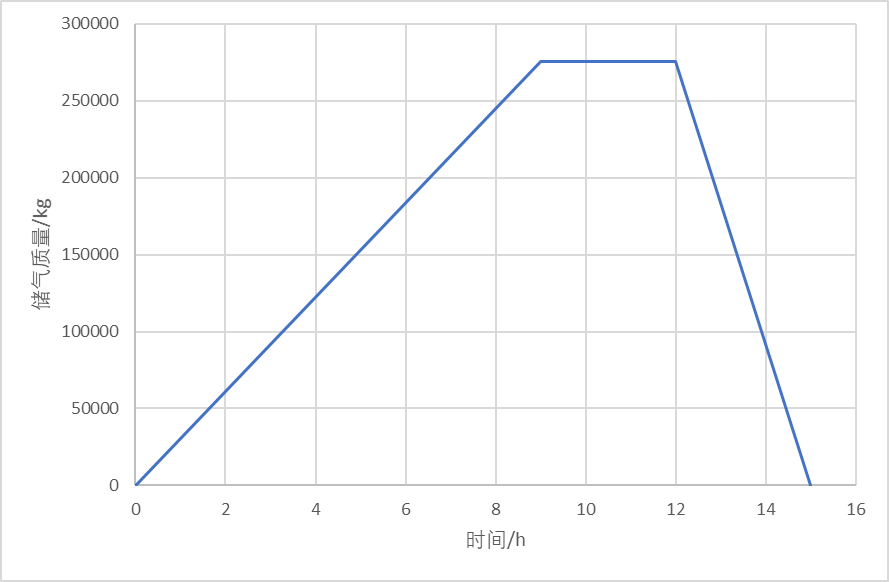
\includegraphics[width=0.9\linewidth]{pictures/screenshot009}
				\label{fig5a}   %以pic.jpg的0.5倍大小输出
			\end{minipage}
		}
		\subfigure[系统设计工况条件下运行一周期的储气装置内压缩空气总体积变化] %第一张子图
		{
			\begin{minipage}{0.5\linewidth}
				\centering          %子图居中
				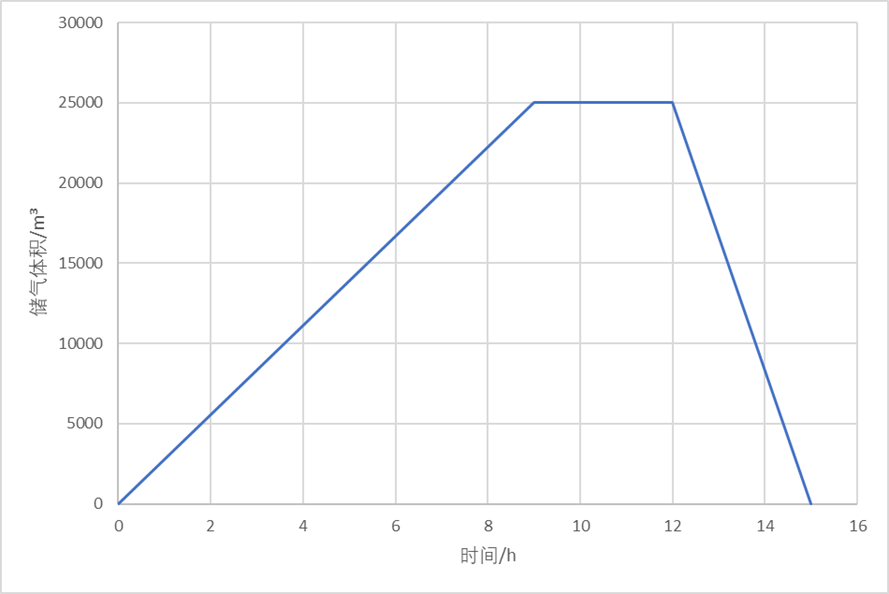
\includegraphics[width=0.9\linewidth]{pictures/screenshot010}
				\label{fig5b}   %以pic.jpg的0.5倍大小输出
			\end{minipage}
		}
		\caption{\fontsize{10.5bp}{10pt}额定工况下储气包的变化} %  %大图名称
		\label{fig:5}  %图片引用标记
	\end{figure}
	
	\par 图$ \fontsize{10.5bp}{10pt}\ref{fig5a} $和图$ \fontsize{10.5bp}{10pt}\ref{fig5b} $分别表示系统在设计工况条件下运行一周期的储气装置内压缩空气总质量和总体积的变化情况,可以看出,气体损失相比于储气装置的储气容量是非常小的,甚至可以忽略不计,换言之,系统的自然放电率小到可以忽略不计,这也是海上风电-水下压缩空气储能互补系统可以作为长期储能系统的重要原因。
	
	\begin{figure}[h]
		\subfigure[系统设计工况条件下运行一周期电动机输入功率和发电机的输出功率变化] %第一张子图
		{
			\begin{minipage}{0.5\linewidth}
				\centering          %子图居中
				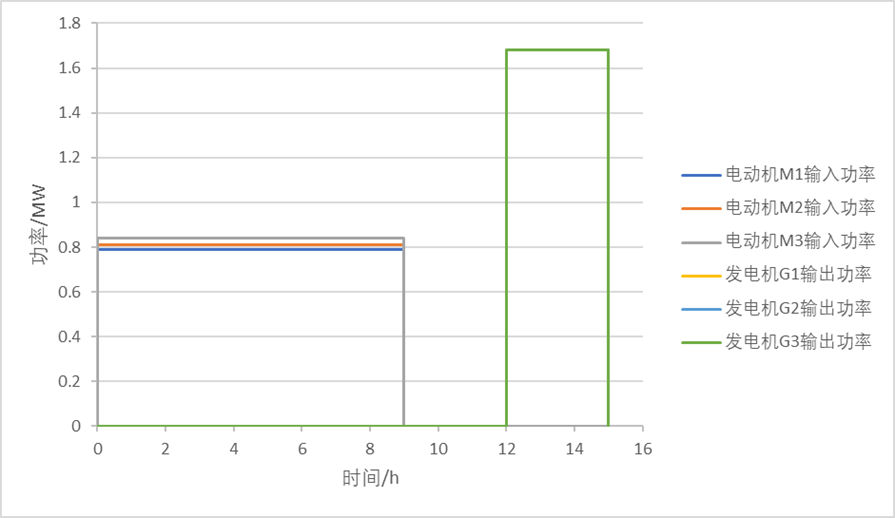
\includegraphics[width=0.9\linewidth]{pictures/screenshot011}
				\label{fig6a}   %以pic.jpg的0.5倍大小输出
			\end{minipage}
		}
		\subfigure[系统设计工况条件下运行一周期空气压缩机压缩效率和空气膨胀机膨胀效率变化] %第一张子图
		{
			\begin{minipage}{0.5\linewidth}
				\centering          %子图居中
				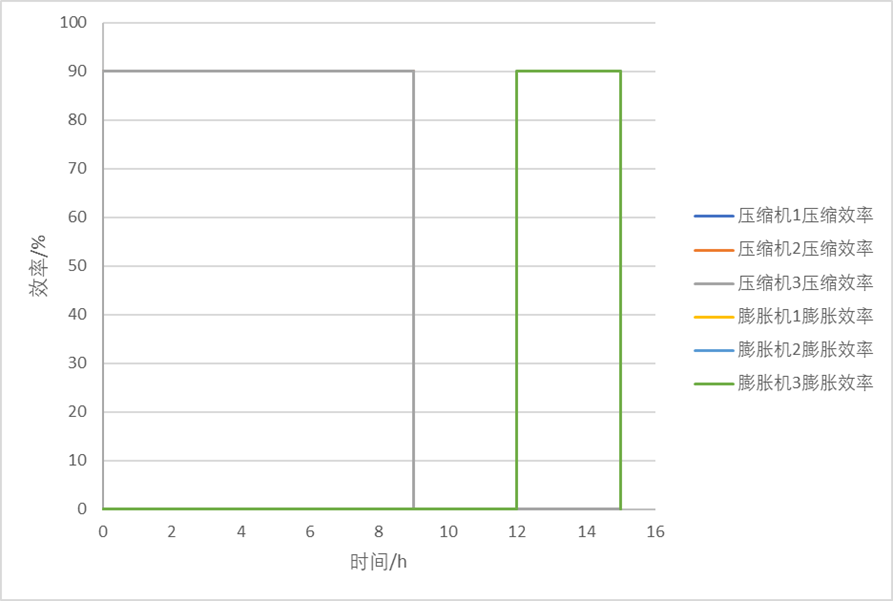
\includegraphics[width=0.9\linewidth]{pictures/screenshot012}
				\label{fig6b}   %以pic.jpg的0.5倍大小输出
			\end{minipage}
		}
		\subfigure[系统设计工况条件下运行一周期高温导热油和低温导热油的质量变化] %第一张子图
		{
			\begin{minipage}{0.5\linewidth}
				\centering          %子图居中
				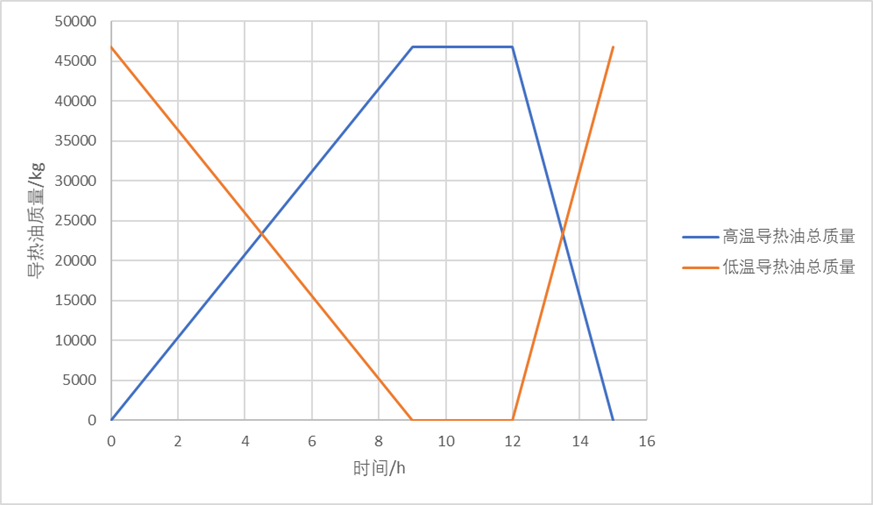
\includegraphics[width=0.9\linewidth]{pictures/screenshot013}
				\label{fig6c}   %以pic.jpg的0.5倍大小输出
			\end{minipage}
		}
		\subfigure[系统设计工况条件下运行一周期系统效率变化] %第一张子图
		{
			\begin{minipage}{0.5\linewidth}
				\centering          %子图居中
				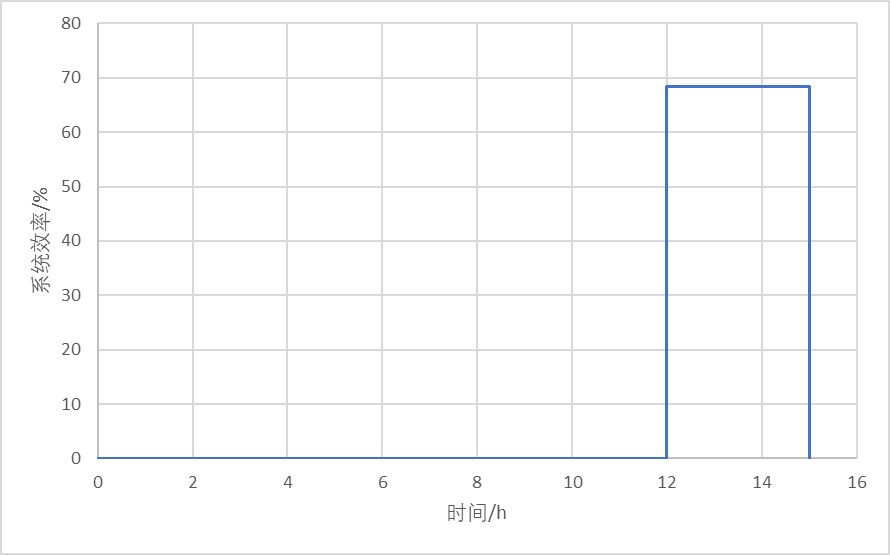
\includegraphics[width=0.9\linewidth]{pictures/screenshot014}
				\label{fig6d}   %以pic.jpg的0.5倍大小输出
			\end{minipage}
		}
		\caption{\fontsize{10.5bp}{10pt}系统设计工况条件下各系统运行情况} %  %大图名称
		\label{fig:6}  %图片引用标记
	\end{figure}
	
	\par 图$ \fontsize{10.5bp}{10pt}\ref{fig6a} $所示为系统在设计工况条件下运行一周期驱动空气压缩机的电动机输入功率和连接空气膨胀机的发电机的输出功率的变化情况,可以看出电动机/发电机功率是基本保持稳定的。
	\par 图$ \fontsize{10.5bp}{10pt}\ref{fig6b} $所示为系统在设计工况条件下运行一周期空气压缩机压缩效率和空气膨胀机膨胀效率的变化,因为是在设计工况条件下,所以压缩机和膨胀机均工作在额定效率下。
	\par 图$ \fontsize{10.5bp}{10pt}\ref{fig6c} $所示为系统在设计工况条件下运行一周期高温导热油和低温导热油的质量变化,因为高温导热油和低温导热油在设计工况条件下稳定循环流动,故二者质量变化曲线是相互对称的。
	\par 图$ \fontsize{10.5bp}{10pt}\ref{fig6d} $所示为系统在设计工况条件下运行一周期的系统效率变化,其表现在膨胀释能过程,设计工况条件下系统效率可达$ 68.46\% $,相比于火力发电厂,水力发电厂,风力发电站等常规发电机构的系统效率而言,系统效率有了极大的提高。
	
	\section{系统变工况运行}
	\subsection{系统变工况分析思路}
	
	\par 根据第3节的热力学模型分析,假设本系统压缩储能过程工作在变工况条件,膨胀释能过程因受控程度比压缩储能过程更高,故膨胀释能过程工作在设计工况条件。以下是压缩储能过程在变工况条件下运行的分析思路。
	\par 
	首先,海上风力发电机组输出功率随海上风速变化而变化的电能,其输出功率范围为$ [0MW,3.06MW] $,电动机$ M1,M2,M3 $分别以$ 32.24\%,33.06\% $和$ 34.7\% $的比例将海上风力发电机组的输出电能划分,如图$ \fontsize{10.5bp}{10pt}\ref{fig7a} $所示为海上风力发电机组实际输出功率与各台电动机实际输入功率的关系图,由表$ \fontsize{10.5bp}{10pt}\ref{tab:my-table} $可知,海上风力发电机组在额定工况条件下的输出值为$ 2.45MW $,电动机$ M1,M2 $和$ M3 $在额定工况条件下的输入值分别为$ 0.79MW,0.81MW $和$ 0.84MW $,以这些数值为基准值,可以得到如图$ \fontsize{10.5bp}{10pt}\ref{fig7b} $所示的海上风力发电机组输出标幺值与各台电动机输入标幺值关系图。
	
	\begin{figure}[h]
		\subfigure[海上风力发电机组实际输出功率与各台电动机实际输入功率的关系] %第一张子图
		{
			\begin{minipage}{0.5\linewidth}
				\centering          %子图居中
				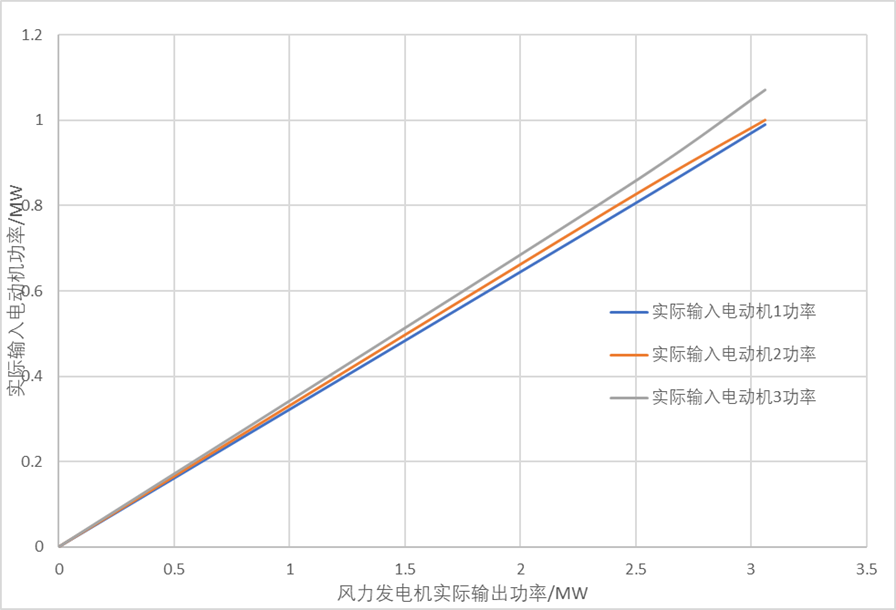
\includegraphics[width=0.9\linewidth]{pictures/screenshot015}
				\label{fig7a}   %以pic.jpg的0.5倍大小输出
			\end{minipage}
		}
		\subfigure[海上风力发电机组输出标幺值与各台电动机输入标幺值关系] %第一张子图
		{
			\begin{minipage}{0.5\linewidth}
				\centering          %子图居中
				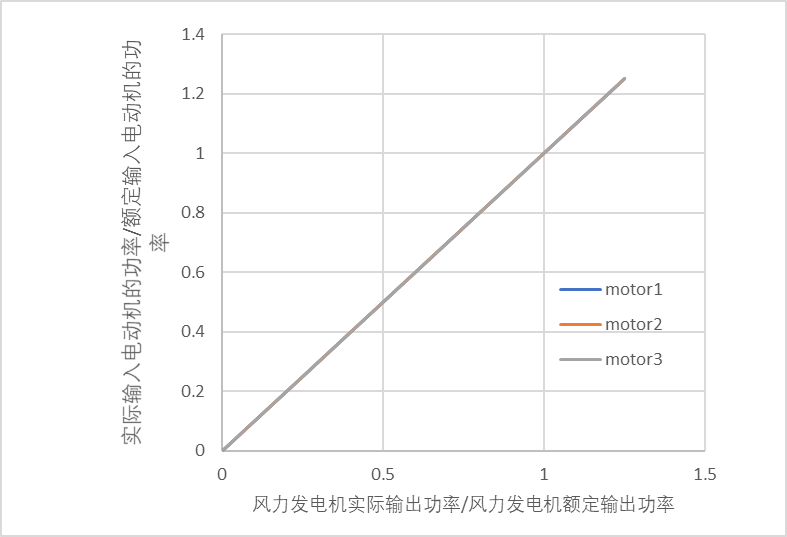
\includegraphics[width=0.9\linewidth]{pictures/screenshot016}
				\label{fig7b}   %以pic.jpg的0.5倍大小输出
			\end{minipage}
		}
		\caption{\fontsize{10.5bp}{10pt}变工况下电动机的输入} %  %大图名称
		\label{fig:7}  %图片引用标记
	\end{figure}
	
	\par 其次,电动机$ M1.M2 $和$ M3 $分别驱动空气压缩机$ C1,C2 $和$ C3 $对空气进行压缩,当电动机实际输入功率变化时,进入空气压缩机的空气质量流量也随之变化,如图$ \fontsize{10.5bp}{10pt}\ref{fig:screenshot017} $所示为电动机输入功率标幺值与空气质量流量标幺值(以$ 8.5kg/s $为基准值)的关系图。
	
	\begin{figure}[H]
		\centering
		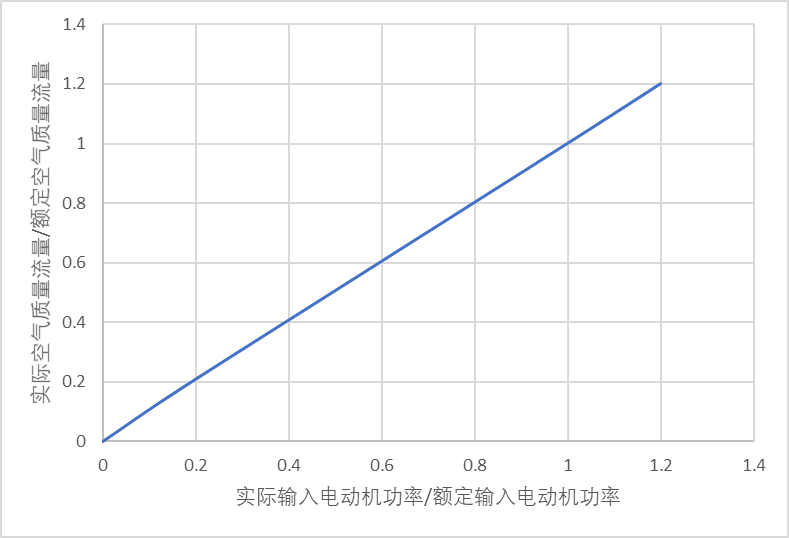
\includegraphics[width=0.7\linewidth]{pictures/screenshot017}
		\caption{\fontsize{10.5bp}{10pt}电动机输入功率标幺值与空气质量流量标幺值(以$ 8.5kg/s $为基准值)的关系图}
		\label{fig:screenshot017}
	\end{figure}
	
	\par 再次,当进入空气压缩机空气质量流量变化时,空气压缩机的压缩效率也随之变化,如图$ \fontsize{10.5bp}{10pt}\ref{fig3b} $所示
	\par 最后,通过观察,不难发现图$ \fontsize{10.5bp}{10pt}\ref{fig7a} $,图$ \fontsize{10.5bp}{10pt}\ref{fig7b} $,图$ \fontsize{10.5bp}{10pt}\ref{fig:screenshot017} $三者存在递进关系,根据这种递进关系,可得出压缩储能过程空气质量流量随时间变化的关系图,对该关系图进行积分运算,结合式$ (\fontsize{10.5bp}{10pt}\ref{f33}) $,即可求解出变工况条件下的系统效率。\\
	
	\subsection{系统变工况分析实例}
	
	\par 根据$ 4.2.1 $的思路,先对压缩储能过程进行一周期$ 24 $小时的实例分析变工况分析。如图$ \fontsize{10.5bp}{10pt}\ref{fig9a} $所示,海上风力发电机组输出为跟随海上风速随机变化的电能,其输出功率范围为$ [0MW,3.06MW] $,其中输出为$ 2.45MW $时为本系统的设计工况点,图$ \fontsize{10.5bp}{10pt}\ref{fig9b} $所示为风力发电机组输出以$ 2.45MW $为基准值的标幺值图形式。\\
	\begin{figure}[H]
		\subfigure[某日0-24时海上风力发电机组输出功率(有名值)] %第一张子图
		{
			\begin{minipage}{0.5\linewidth}
				\centering          %子图居中
				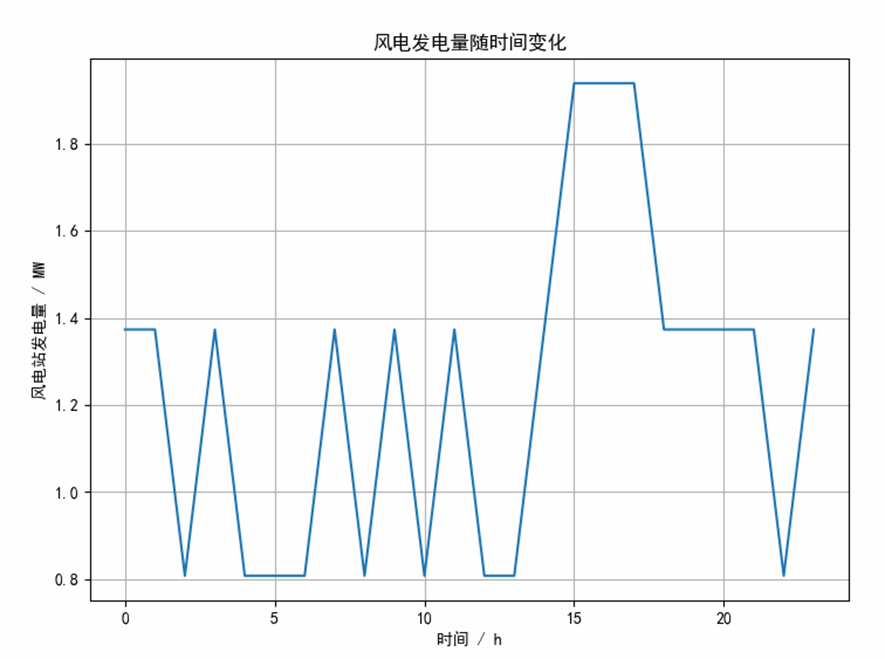
\includegraphics[width=0.9\linewidth]{pictures/screenshot019}
				\label{fig9a}   %以pic.jpg的0.5倍大小输出
			\end{minipage}
		}
		\subfigure[某日0-24时海上风力发电机组输出功率(标幺值)] %第一张子图
		{
			\begin{minipage}{0.5\linewidth}
				\centering          %子图居中
				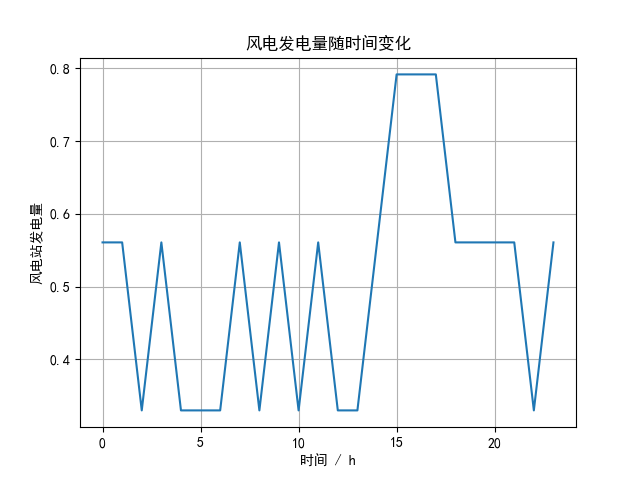
\includegraphics[width=0.9\linewidth]{pictures/screenshot018}
				\label{fig9b}   %以pic.jpg的0.5倍大小输出
			\end{minipage}
		}
		\caption{\fontsize{10.5bp}{10pt}风电站} %  %大图名称
		\label{fig:9}  %图片引用标记
	\end{figure}
	
	\par 电动机$ M1,M2 $和$ M3 $所输入的电能比分别为$ 32.24\%,33.06\% $和$ 34.7\% $,图$ \fontsize{10.5bp}{10pt}\ref{fig10a} $和$ \fontsize{10.5bp}{10pt}\ref{fig10b} $分别为$ 3 $台电动机输入功率的有名值图和标幺值图(基准值分别为$ 0.79MW,0.81MW$和$ 0.84MW $)。\\
	\begin{figure}[H]
		\subfigure[某日0-24时三台电动机输入功率(有名值)] %第一张子图
		{
			\begin{minipage}{0.5\linewidth}
				\centering          %子图居中
				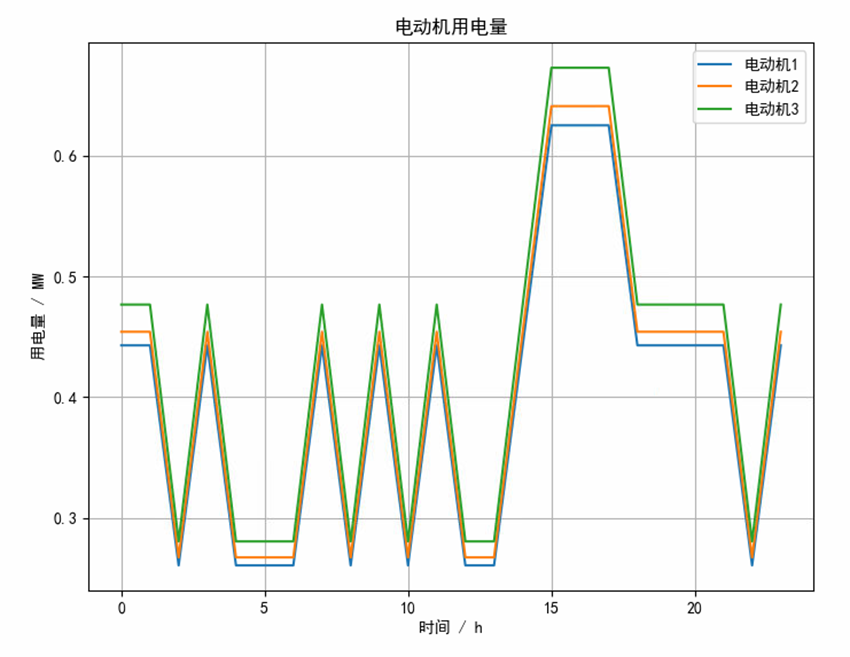
\includegraphics[width=0.9\linewidth]{pictures/screenshot020}
				\label{fig10a}   %以pic.jpg的0.5倍大小输出
			\end{minipage}
		}
		\subfigure[某日0-24时三台电动机输入功率(标幺值)] %第一张子图
		{
			\begin{minipage}{0.5\linewidth}
				\centering          %子图居中
				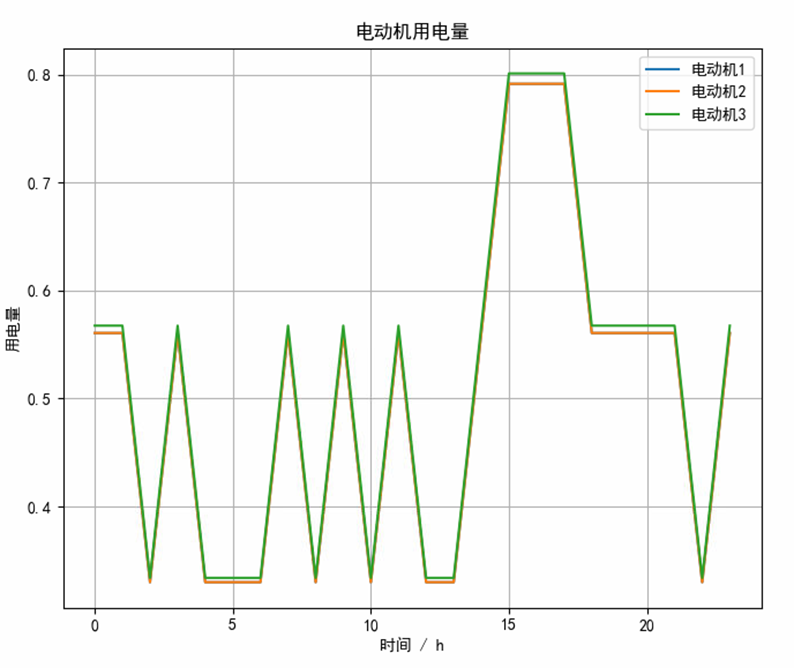
\includegraphics[width=0.9\linewidth]{pictures/screenshot021}
				\label{fig10b}   %以pic.jpg的0.5倍大小输出
			\end{minipage}
		}
		\caption{\fontsize{10.5bp}{10pt}电动机} %  %大图名称
		\label{fig:10}  %图片引用标记
	\end{figure}
	
	\par 电动机$ M1,M2 $和$ M3 $驱动空气压缩机$ C1,C2 $和$ C3 $对空气进行三级压缩,因电动机输入功率随时间变化,故进入压缩机的空气质量流量也随时间变化,图$ \fontsize{10.5bp}{10pt}\ref{fig11a} $和图$ \fontsize{10.5bp}{10pt}\ref{fig11b} $所示分别为空气质量流量随时间变化的标幺值图(基准值为$ 8.5kg/s $)和有名值图。\\
	\begin{figure}[H]
		\subfigure[某日0-24时空气质量流量变化(有名值)] %第一张子图
		{
			\begin{minipage}{0.5\linewidth}
				\centering          %子图居中
				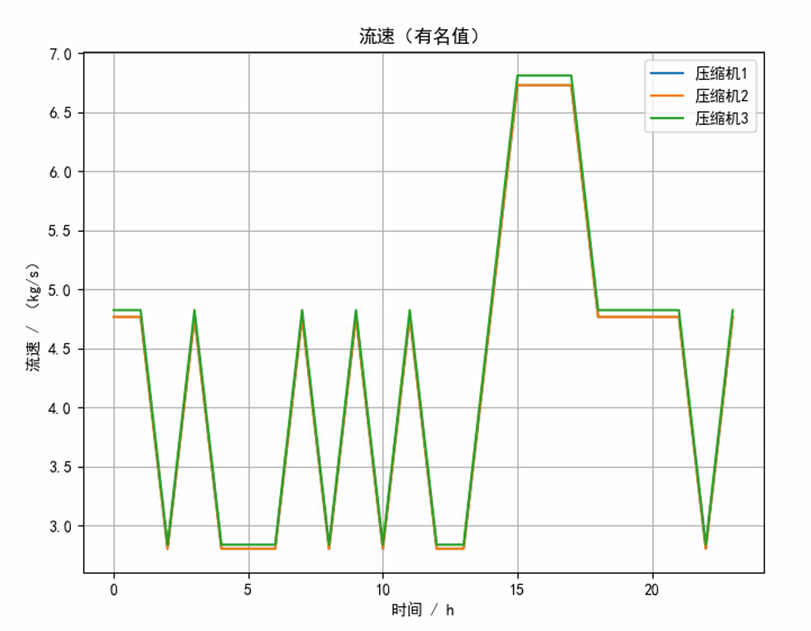
\includegraphics[width=0.9\linewidth]{pictures/screenshot022}
				\label{fig11a}   %以pic.jpg的0.5倍大小输出
			\end{minipage}
		}
		\subfigure[某日0-24时空气质量流量变化(标幺值)] %第一张子图
		{
			\begin{minipage}{0.5\linewidth}
				\centering          %子图居中
				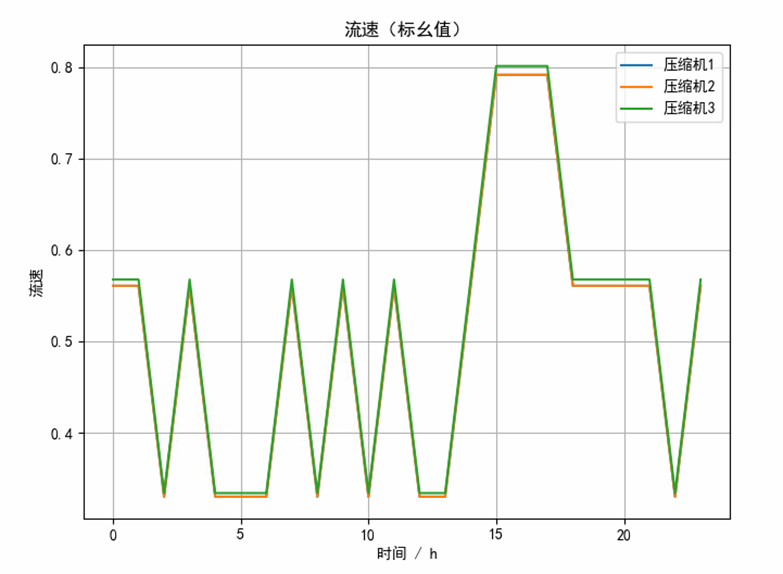
\includegraphics[width=0.9\linewidth]{pictures/screenshot023}
				\label{fig11b}   %以pic.jpg的0.5倍大小输出
			\end{minipage}
		}
		\caption{\fontsize{10.5bp}{10pt}空气质量流量} %  %大图名称
		\label{fig:11}  %图片引用标记
	\end{figure}
	
	\par 如图$ \fontsize{10.5bp}{10pt}\ref{fig12a} $因受空气质量流量变化的影响,故三台压缩机的压缩效率也表现为随时间变化,压缩效率变化,进而导致压缩终温和高温导热油温度变化。
	\begin{figure}[H]
		\centering
		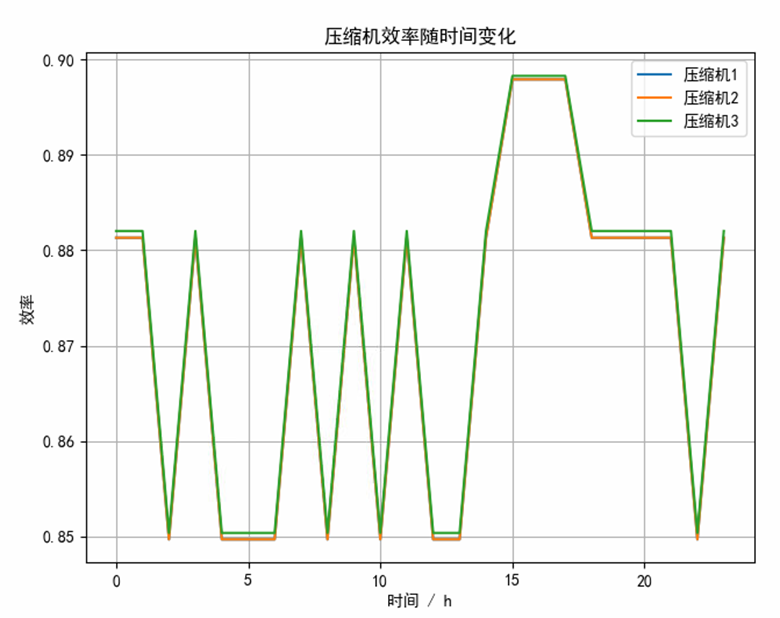
\includegraphics[width=0.7\linewidth]{pictures/screenshot024}
		\caption{\fontsize{10.5bp}{10pt}某日0-24时三台压缩机压缩效率变化}
		\label{fig12a}
	\end{figure}
	
	\par 将图$ \fontsize{10.5bp}{10pt}\ref{fig9a} $风电站输出功率和图$ \fontsize{10.5bp}{10pt}\ref{fig11a} $空气质量流量分别对时间积分,得到如图$ \fontsize{10.5bp}{10pt}\ref{fig12b} $所示的海上风力发电机组总发电量与时间的关系图和图$ \fontsize{10.5bp}{10pt}\ref{fig12c} $所示的储气包储存空气总质量与时间的关系图。
	\begin{figure}[H]
		\subfigure[某日0-24时风力发电机组总发电量变化] %第一张子图
		{
			\begin{minipage}{0.5\linewidth}
				\centering          %子图居中
				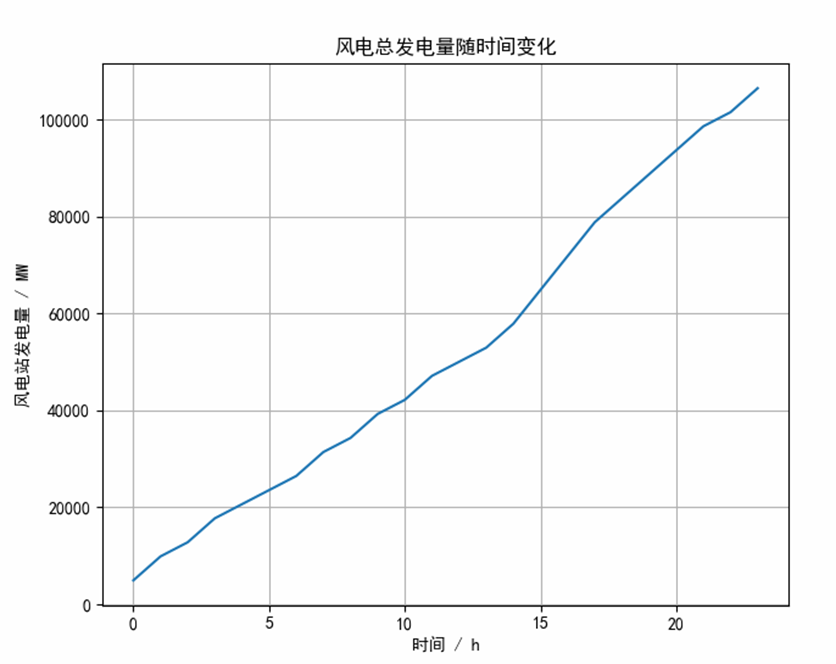
\includegraphics[width=0.9\linewidth]{pictures/screenshot025}
				\label{fig12b}   %以pic.jpg的0.5倍大小输出
			\end{minipage}
		}
		\subfigure[某日0-24时储气包内压缩空气总质量变化] %第一张子图
		{
			\begin{minipage}{0.5\linewidth}
				\centering          %子图居中
				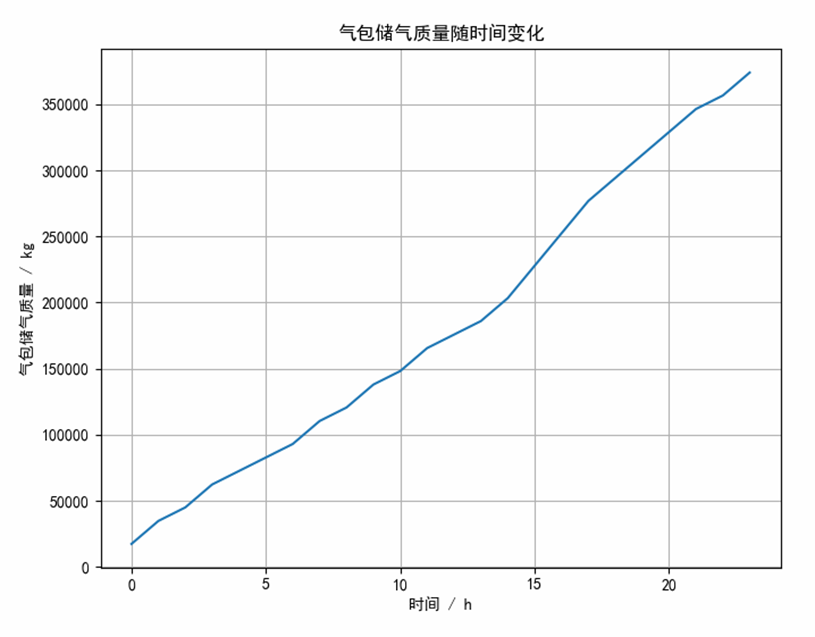
\includegraphics[width=0.9\linewidth]{pictures/screenshot026}
				\label{fig12c}   %以pic.jpg的0.5倍大小输出
			\end{minipage}
		}
		\caption{\fontsize{10.5bp}{10pt}积分结果} %  %大图名称
		\label{fig:13}  %图片引用标记
	\end{figure}
	
	\par 根据数据统计,工业用电和居民用电高峰期为每日$ 18:00-23:00 $,因此规定本系统压缩储能时段为每日$ 0:00-15:00 $,高压空气存储时段为每日$ 15:00-18:00 $,膨胀释能时段为每日$ 18:00-20:30 $。这样规定的目的是在非用电高峰期进行压缩储能,用电高峰期膨胀释能来使得本系统输出的电能最大化地被利用,减轻其它常规发电机构的负荷。每日$ 15:00-18:00 $位高压空气储存阶段,该阶段内储气包空气气压损失忽略不计,每日$ 18:00-20:30 $为膨胀释能时段,膨胀释能过程运行在系统设计工况条件下,图$ \ref{fig14a} $所示为储存高压空气时段和膨胀释能时段储气包内空气质量变化与时间的关系图,图$ \ref{fig14b} $所示为膨胀释能时段发电机$ G1,G2,G3 $输出功率与时间的关系图。综合上述分析,可得表$ \fontsize{10.5bp}{10pt}\ref{tab:my-table2} $所示的各时段相关参数。根据表$ \fontsize{10.5bp}{10pt}\ref{tab:my-table2} $数据和式$ (\fontsize{10.5bp}{10pt}\ref{f33}) $可得,系统效率$ \eta_{system}=\frac{48060}{69652} \times 100\%=69\% $。
	
	\begin{figure}[H]
		\subfigure[储存空气和膨胀释能时段储气包内压缩空气总质量变化] %第一张子图
		{
			\begin{minipage}{0.5\linewidth}
				\centering          %子图居中
				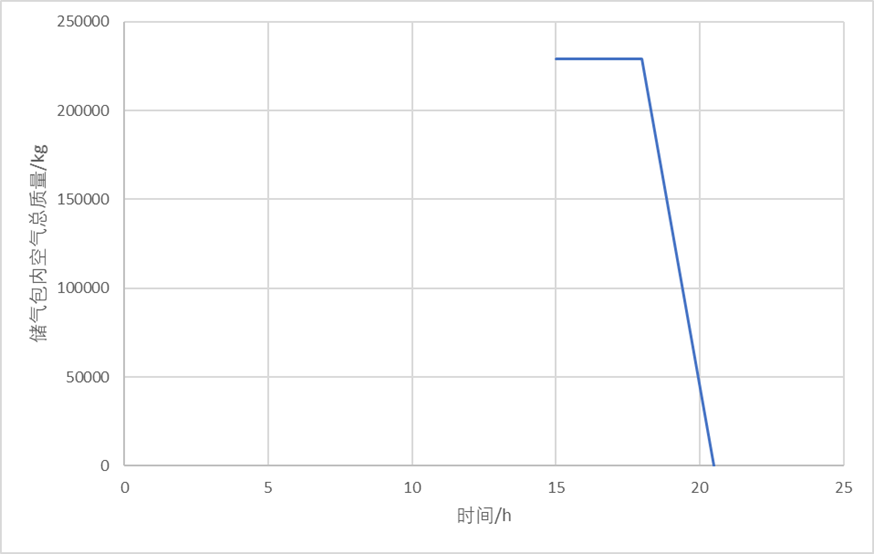
\includegraphics[width=0.9\linewidth]{pictures/screenshot027}
				\label{fig14a}   %以pic.jpg的0.5倍大小输出
			\end{minipage}
		}
		\subfigure[膨胀释能时段三台发电机输出功率变化] %第一张子图
		{
			\begin{minipage}{0.5\linewidth}
				\centering          %子图居中
				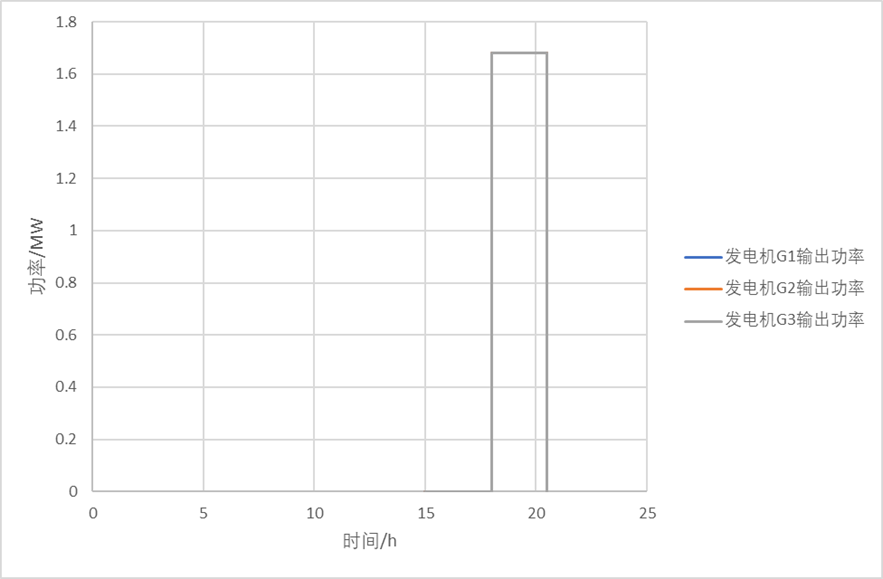
\includegraphics[width=0.9\linewidth]{pictures/screenshot028}
				\label{fig14b}   %以pic.jpg的0.5倍大小输出
			\end{minipage}
		}
		\caption{\fontsize{10.5bp}{10pt}膨胀过程} %  %大图名称
		\label{fig:14}  %图片引用标记
	\end{figure}
	
	\begin{table}[H]
		\resizebox{\textwidth}{!}{
			\begin{tabular}{|c|c|r|r|r|r|r|r|}
				\hline
				\multicolumn{1}{|l|}{过程} & \multicolumn{1}{l|}{时段} & \multicolumn{1}{l|}{本时段海上风力}  & \multicolumn{1}{l|}{储气包储气} & \multicolumn{1}{l|}{发电机G1} & \multicolumn{1}{l|}{发电机G2} & \multicolumn{1}{l|}{发电机G3} & \multicolumn{1}{l|}{本时段内发电机}     \\
				\multicolumn{1}{|l|}{}   & \multicolumn{1}{l|}{}   & \multicolumn{1}{l|}{发电机组总发电量} & \multicolumn{1}{l|}{总质量}   & \multicolumn{1}{l|}{输出功率}  & \multicolumn{1}{l|}{输出功率}  & \multicolumn{1}{l|}{输出功率}  & \multicolumn{1}{l|}{G1G2G3输出总电能} \\ \hline
				压缩储能                     & 0:00-15:00              & 69652MW                       & 229500kg                   & 0                          & 0                          & 0                          & 0                                \\ \hline
				储存空气                     & 15:00-18:00             & 0                             & 229500kg                   & 0                          & 0                          & 0                          & 0                                \\ \hline
				膨胀时能                     & 18:00-20:30             & 0                             &                            & 1.78MW                     & 1.78MW                     & 1.78MW                     & 48060MW                          \\ \hline
			\end{tabular}
		}
		\caption{\fontsize{10.5bp}{10pt}系统变工况条件下运行各时段发电量}
		\label{tab:my-table2}
	\end{table}
	
	
	\chapter{系统经济效益分析}
	
	\par 根据$ 4.2.2 $变工况实例分析结果,本节主要是对海上风力发电-水下压缩空气储能互补系统进行长远性的经济效益分析,并以此作为该系统可行性的重要依据。
	\par 首先讨论系统运行的成本问题。本系统所需成本主要由$ 4 $个方面组成:
	\begin{enumerate}
		\item 系统部件购买成本
		\item 系统部件安装成本
		\item 系统部件维护保养成本
		\item 系统部件故障维修成本
	\end{enumerate}
	
	\par 依据当前机械市场数据,其具体所需金额如表$ \fontsize{10.5bp}{10pt}\ref{tab:my-table5} $所示。因为该系统是关系到国民经济发展的能源系统,故系统所有部件划分为特种机械范畴,根据《$ TSG $特种设备安全技术规范》规定,系统自运行起每月需进行一次维护保养,其费用约为$ 24980 $元/整系统次。至于故障维修成本是这样规定的,根据特种设备月故障次数函数拟合图$ \fontsize{10.5bp}{10pt}\ref{fig15a} $所示,计算出如图$ \fontsize{10.5bp}{10pt}\ref{fig15b} $所示的日故障概率图,并在系统模型中调用随机函数随机得出设备在规定运行年限内的故障次数,并规定故障维修费用为$ 48400 $元/次。\\
	
	% Please add the following required packages to your document preamble:
	% \usepackage{multirow}
	% \usepackage{graphicx}
	\begin{table}[H]
		\resizebox{\textwidth}{!}{
			\begin{tabular}{|l|r|r|r|r|c|c|}
				\hline
				\multicolumn{1}{|c|}{环节} &
				\multicolumn{1}{c|}{所需容量} &
				\multicolumn{1}{c|}{单价} &
				\multicolumn{1}{c|}{成本/元} &
				\multicolumn{1}{c|}{安装费用/元} &
				维护保养费用/(元/整系统·次) &
				故障维修费用/(元/次) \\ \hline
				风力发电机 &
				5MW &
				1000元/kW &
				5000000 &
				500000 &
				{}{}{24980} &
				{}{}{48600} \\ \cline{1-5}
				电动机M1   & 1MW     & 200元/kW   & 200000   & 20000   &  &  \\ \cline{1-5}
				电动机M2   & 1MW     & 200元/kW   & 200000   & 20000   &  &  \\ \cline{1-5}
				电动机M3   & 1MW     & 200元/kW   & 200000   & 20000   &  &  \\ \cline{1-5}
				空气压缩机1  & 1MW     & 600元/kW   & 600000   & 60000   &  &  \\ \cline{1-5}
				空气压缩机2  & 1MW     & 600元/kW   & 600000   & 60000   &  &  \\ \cline{1-5}
				空气压缩机3  & 1MW     & 600元/kW   & 600000   & 60000   &  &  \\ \cline{1-5}
				空气膨胀机1  & 2MW     & 600元/kW   & 1200000  & 120000  &  &  \\ \cline{1-5}
				空气膨胀机2  & 2MW     & 600元/kW   & 1200000  & 120000  &  &  \\ \cline{1-5}
				空气膨胀机3  & 2MW     & 600元/kW   & 1200000  & 120000  &  &  \\ \cline{1-5}
				发电机G1   & 2MW     & 500元/kW   & 1000000  & 100000  &  &  \\ \cline{1-5}
				发电机G2   & 2MW     & 500元/kW   & 1000000  & 100000  &  &  \\ \cline{1-5}
				发电机G3   & 2MW     & 500元/kW   & 1000000  & 100000  &  &  \\ \cline{1-5}
				换热器1    & -       & 100000元/台 & 100000   & 10000   &  &  \\ \cline{1-5}
				换热器2    & -       & 100000元/台 & 100000   & 10000   &  &  \\ \cline{1-5}
				换热器3    & -       & 100000元/台 & 100000   & 10000   &  &  \\ \cline{1-5}
				换热器4    & -       & 100000元/台 & 100000   & 10000   &  &  \\ \cline{1-5}
				换热器5    & -       & 100000元/台 & 100000   & 10000   &  &  \\ \cline{1-5}
				换热器6    & -       & 100000元/台 & 100000   & 10000   &  &  \\ \cline{1-5}
				柔性储气包   & 30000m³ & 300元/m³   & 9000000  & 900000  &  &  \\ \cline{1-5}
				管路,线路连接 & -       & -         & 1760000  & 23600   &  &  \\ \cline{1-5}
				热液罐     & -       & 100000元/个 & 100000   & 10000   &  &  \\ \cline{1-5}
				冷液罐     & -       & 100000元/个 & 100000   & 10000   &  &  \\ \cline{1-5}
				合计      & -       & -         & 25560000 & 2403600 &  &  \\ \hline
			\end{tabular}
		}
		\caption{\fontsize{10.5bp}{10pt}系统运行成本}
		\label{tab:my-table5}
	\end{table}
	\begin{figure}[H]
		\subfigure[特种设备月故障次数函数拟合图] %第一张子图
		{
			\begin{minipage}{0.5\linewidth}
				\centering          %子图居中
				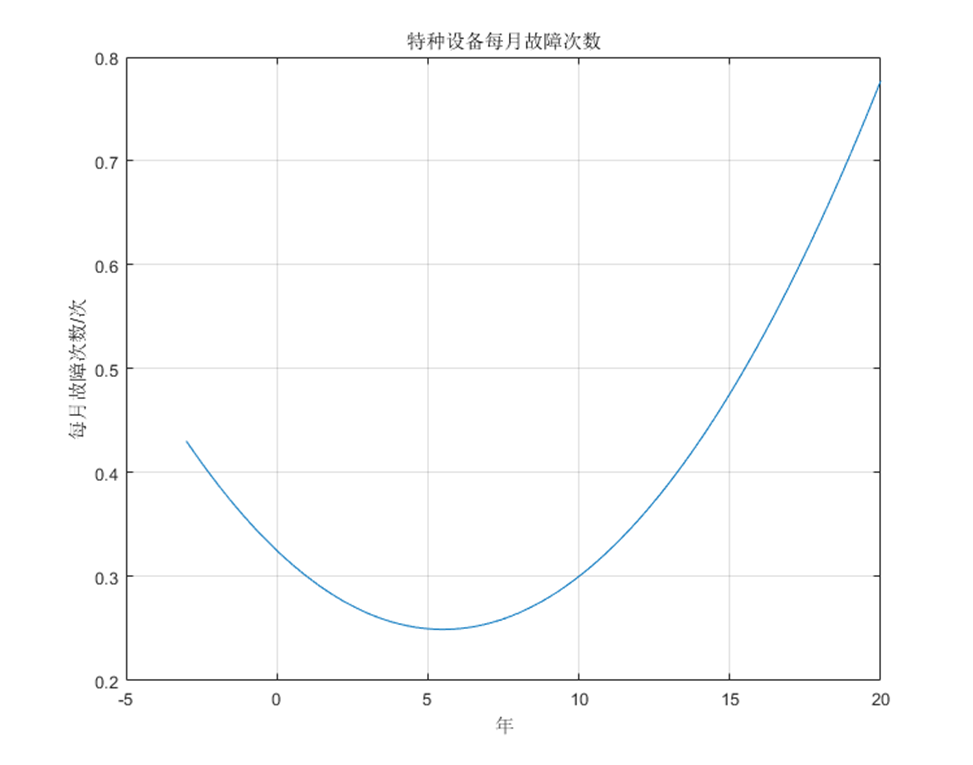
\includegraphics[width=0.9\linewidth]{pictures/screenshot029}
				\label{fig15a}   %以pic.jpg的0.5倍大小输出
			\end{minipage}
		}
		\subfigure[特种设备日故障概率图] %第一张子图
		{
			\begin{minipage}{0.5\linewidth}
				\centering          %子图居中
				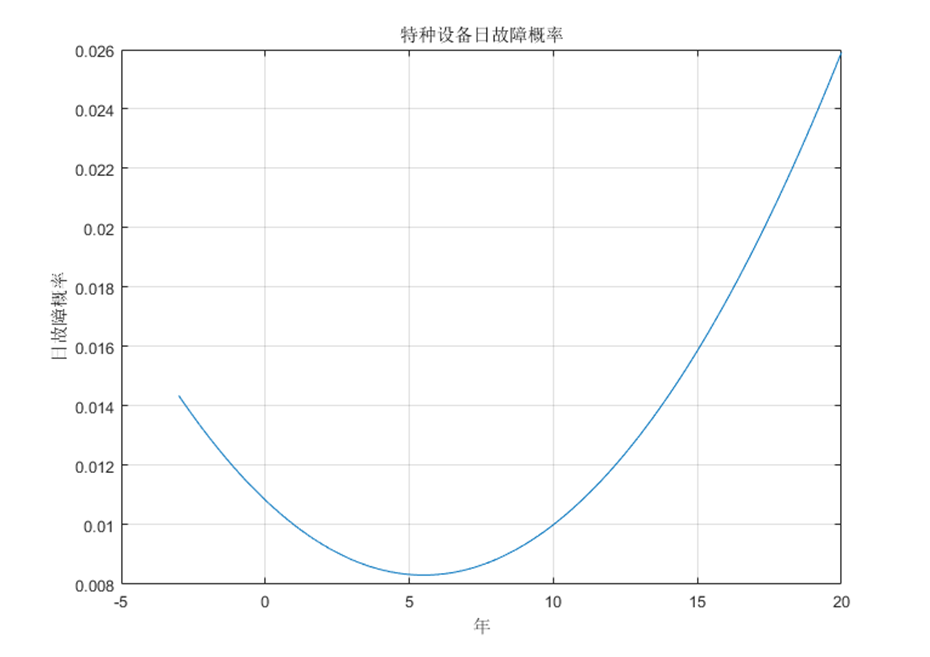
\includegraphics[width=0.9\linewidth]{pictures/screenshot030}
				\label{fig15b}   %以pic.jpg的0.5倍大小输出
			\end{minipage}
		}
		\caption{\fontsize{10.5bp}{10pt}特种设备日故障次数及概率} %  %大图名称
		\label{fig:15}  %图片引用标记
	\end{figure}
	
	
	
	\begin{table}[H]
		\centering
		\resizebox{0.5\textwidth}{!}{
			\begin{tabular}{|l|r|r|}
				\hline
				用电类型                       & \multicolumn{1}{l|}{用电比例} & \multicolumn{1}{l|}{单价/(元/KWh)} \\ \hline
				工业用电                       & 78\%                      & 0.62                            \\ \hline
				\multicolumn{1}{|c|}{居民用电} & 22\%                      & 1.025                           \\ \hline
			\end{tabular}
		}
		\caption{\fontsize{10.5bp}{10pt}18:00-20:30用电类型占比及单价}
		\label{tab:my-table3}
	\end{table}
	
	% Please add the following required packages to your document preamble:
	% \usepackage{graphicx}
	
	\begin{table}[H]
		\centering
		\resizebox{0.8\textwidth}{!}{%
			\begin{tabular}{|l|l|l|l|l|l|}
				\hline
				\begin{tabular}[c]{@{}l@{}}发电总\\ 功率/kW\end{tabular} &
				\begin{tabular}[c]{@{}l@{}}日发电\\ 时长/h\end{tabular} &
				\begin{tabular}[c]{@{}l@{}}日发电\\ 量/kWh\end{tabular} &
				\begin{tabular}[c]{@{}l@{}}工业用电\\ 收入/(元/日)\end{tabular} &
				\begin{tabular}[c]{@{}l@{}}居民用电\\ 收入/(元/日)\end{tabular} &
				收入/(元/日) \\ \hline
				\multicolumn{1}{|r|}{5040} &
				\multicolumn{1}{r|}{2.5} &
				\multicolumn{1}{r|}{12600} &
				\multicolumn{1}{r|}{9326} &
				\multicolumn{1}{r|}{2630} &
				\multicolumn{1}{r|}{11865} \\ \hline
			\end{tabular}%
		}
		\caption{\fontsize{10.5bp}{10pt}系统无故障条件下的日发电量及日收入}
		\label{tab:my-table4}
	\end{table}
	
	\par 其次讨论系统运行的收入问题,根据参考文献\cite{b4}得知本系统的发电时段$ 18:00-20:30 $所处的用电高峰期内居民用电占比约为$ 22\% $,工业用电占比为$ 78\% $,珠海市电单价如表$ \fontsize{10.5bp}{10pt}\ref{tab:my-table3} $所示。参考表$ \fontsize{10.5bp}{10pt}\ref{tab:my-table2} $数据,可得表$ \fontsize{10.5bp}{10pt}\ref{tab:my-table4} $所示的系统无故障条件下的日发电量及日收入数据。并规定若当日系统发生故障,并且当日无收入。\\
	
	\par 将成本计算方法和日收入计算方法输入到系统模型中,得到如图$ \fontsize{10.5bp}{10pt}\ref{fig:screenshot031} $所示的系统运行成本、总收入、净收入变化图。通过观察图$ \fontsize{10.5bp}{10pt}\ref{fig:screenshot031} $,发现系统运行月$ 9.58 $年时,开始盈利,在特种机械有效寿命$ 20 $年内,总净收入可达$ 2.81 $千万元。
	
	\begin{figure}[H]
		\centering
		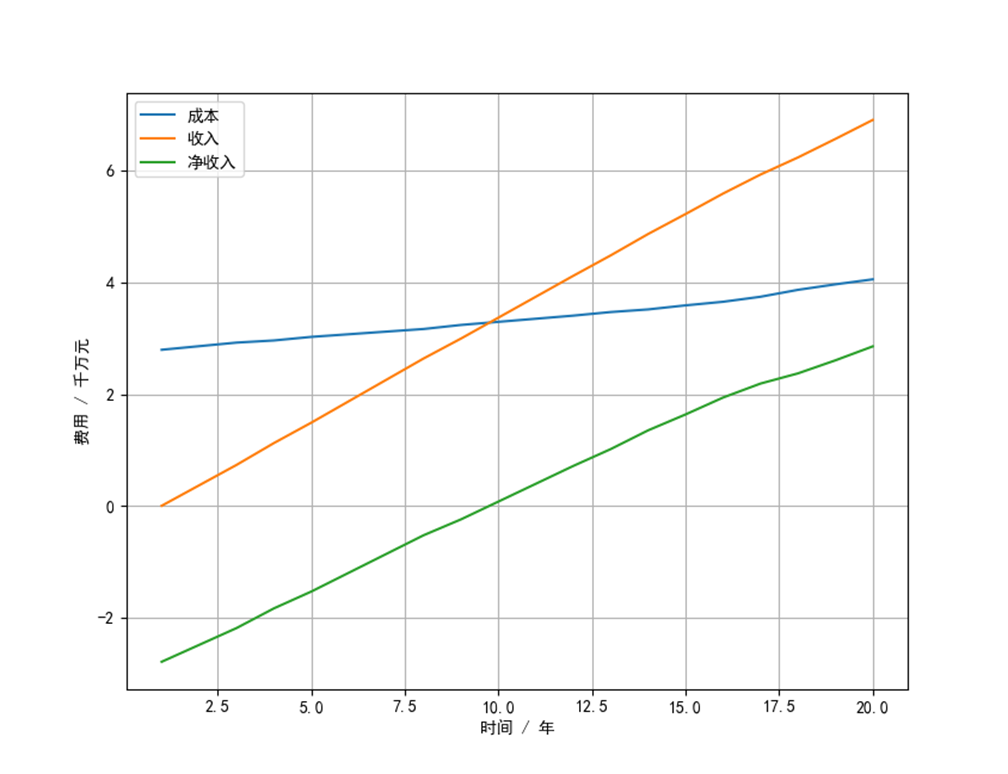
\includegraphics[width=0.7\linewidth]{pictures/screenshot031}
		\caption{\fontsize{10.5bp}{10pt}系统运行成本、总收入、净收入变化}
		\label{fig:screenshot031}
	\end{figure}
	
	\chapter*{结论}
	
	\par 本文围绕所设计的海上风力发电-水下压缩空气储能互补系统进行能效分析和经济效益分析,综合考虑了该新能源系统的能源利用有效性、经济性和可实现性等多方面问题。系统模型的仿真结果显示,借助海上风力发电机组、空气压缩机、柔性储气包、空气膨胀机、换热器等主要机械部件构成的海上风力发电-水下压缩空气互补系统可以将随机性强波动性大的海上风能先转化为稳定的物质内能,再转化为稳定输出的电能,实现了能量从不稳定输出到稳定输出的转变,相比于传统的风力发电,大大减小了能源系统输出电能对电网的冲击,保障了电网、国民经济生产和人民生活用电的安全。同时,将柔性储气包设置在海洋$ 100m $左右的环境时,在风速随机波动条件下系统效率仍可达$ 69\% $,且安装难度较小和安装成本较低,整个系统在有效寿命$ 20 $年期限内可获得近$ 2.85 $千万元的总利润,做到了系统能效性和经济性的统一,为系统的可实现性提供了重要依据,供相关能源部门决策参考。
	
	
	
	\begin{thebibliography}{100}
		%引用用\cite
		\bibitem{b5}
		贾涛,王兴月. \emph{海洋平台多能互补系统电源容量优化}. [J].\hskip 1em plus
		0.5em minus 0.4em\relax 太重(天津)滨海重型机械有限公司技术中心. 2017. 
		
		\bibitem{b4}
		李建民. \emph{夏季用电高峰期间电气设备运行重点}. [J].\hskip 1em plus
		0.5em minus 0.4em\relax 北京电力亦庄供电公司. 2006. 
		
		\bibitem{b1}
		王志文. \emph{水下压缩空气储能系统设计与能效分析}. [D].\hskip 1em plus
		0.5em minus 0.4em\relax 大连海事大学. 2017.
		
		\bibitem{b2}
		王志文,熊伟,王海涛,王祖温. \emph{水下压缩空气储能研究进展}. [J].\hskip 1em plus
		0.5em minus 0.4em\relax 大连海事大学船舶机电装备研究所. 2015.
		
		\bibitem{b8}
		闫晔. \emph{考虑风电不确定性的分时电价研究}. [D].\hskip 1em plus
		0.5em minus 0.4em\relax 西安理工大学. 2020.
		
		\bibitem{b6}
		Brian C. Cheung, Rupp Carriveau, David S.K. Ting. \emph{Multi-objective optimization of an underwater compressed air energy
			storage system using genetic algorithm}. [J].\hskip 1em plus
		0.5em minus 0.4em\relax Turbulence and Energy Laboratory, Ed Lumley Centre for Engineering Innovation, University of Windsor. 2014. 
		
		\bibitem{b7}
		F. Fornarelli, S.M. Camporeale, B. Fortunato, M. Torresi, P. Oresta, L. Magliocchetti, A. Miliozzi,
		G. Santo
		. \emph{CFD analysis of melting process in a shell-and-tube latent heat storage
			for concentrated solar power plants}. [J].\hskip 1em plus
		0.5em minus 0.4em\relax a Politecnico di Bari, Dipartimento di Ingegneria Meccanica, Matematica e Management, Sezione di Macchine ed Energetica, Via Orabona 4, 70125 Bari, Italy. 2016. 
		
		\bibitem{b3}
		Wolf D. \emph{Methods for Design and Application of Adiabatic Compressed Air Energy Storage Based on Dynamic Modeling}. [D].\hskip 1em plus
		0.5em minus 0.4em\relax Ruhr-Universitat Bochum. 2010. 
		
		
		
		
		
	\end{thebibliography}
	%\end{multicols}
	
	
	
\end{document}